\documentclass[twoside]{ctuthesis}
\usepackage{graphicx}
\usepackage{adjustbox}
\usepackage{makecell}
\usepackage[colorinlistoftodos]{todonotes}
\usepackage[sortlocale=cs_CZ, sorting=debug, style=iso-numeric, maxnames=2]{biblatex}
\usepackage{array,etoolbox}
\usepackage{xcolor}
\usepackage{caption}
\usepackage{subcaption}
\usepackage{enumitem}
\usepackage{multirow}
\usepackage{multicol}
\usepackage{chngpage}
\usepackage{rotating}
\usepackage{empheq}
\usepackage{color, colortbl}
\usepackage[acronym,nomain,nonumberlist]{glossaries}
\makenoidxglossaries

\renewcommand{\glossarysection}[2][]{}

\newacronym{ui}{UI}{User Interface}
\newacronym{os}{OS}{Operační systém}
\newacronym{dpp}{DPP}{Dohoda o~provedení práce}
\newacronym{dpc}{DPČ}{Dohoda o~pracovní činnosti}
\newacronym{mvc}{MVC}{Model-View-Controller}
\newacronym{mvvm}{MVVM}{Model-View-ViewModel}
\newacronym{uc}{UC}{Use Case}
\newacronym{dao}{DAO}{Data Access Object}
\newacronym{rest}{REST}{Representational state transfer}
\newacronym{api}{API}{Application Programming Interface}
\newacronym{paas}{PaaS}{Platform as a Service}
\newacronym{dbms}{DBMS}{Database Management System}

\newacronym{json}{JSON}{JavaScript Object Notation}
\newacronym{crud}{CRUD}{Create, Read, Update, Delete}
\newacronym{html}{HTML}{Hypertext Markup Language}
\newacronym{css}{CSS}{Cascading Style Sheets}
\newacronym{xml}{XML}{Extensible Markup Language}
\newacronym{sql}{SQL}{Structured Query Language}
\newacronym{orm}{ORM}{Object Relation Mapping}
\newacronym{id}{ID}{Identifikátor}

\newacronym{dsl}{DSL}{Domain-specific language}
\newacronym{http}{HTTP}{Hypertext Transfer Protocol}
\newacronym{url}{URL}{Uniform Resource Locator}
\newacronym{mvp}{MVP}{Model-View-Presenter}
\newacronym{ide}{IDE}{Integrated Development Environment}

\newacronym{rpc}{RPC}{Remote Procedure Call}
\newacronym{erp}{ERP}{Enterprise Resource Planning}

\usepackage{listings}

\definecolor{Gray}{gray}{0.9}

\newcommand{\coloredeq}[2]{\begin{empheq}[box=\colorbox{Gray}]{align}\label{#1}\hspace{1em}#2\hspace{1em}\end{empheq}}

\graphicspath{{img/}}

\preto\tabular{\setcounter{magicrownumbers}{0}}
\newcounter{magicrownumbers}
\newcommand\rownumber{\stepcounter{magicrownumbers}\arabic{magicrownumbers}}

\renewcommand*{\finalnamedelim}{ a }

\ctusetup{
	mainlanguage = czech,
	otherlanguages = {slovak, english},
	title-czech = {Mobilní aplikace pro plánování lidských zdrojů},
	title-english = {Mobile App for Human Resource Planning},
	doctype = B,
	faculty = F3,
	department-czech = {Katedra počítačů},
	department-english = {Department of Computer Science},
	author = {Martina Kopecká},
	supervisor = {Ing. Jiří Šebek},
	supervisor-address = {},
	fieldofstudy-english = {Software Engineering -- TODO, co je ENG nazev},
	fieldofstudy-czech = {Softwarové inženýrství a technologie},
	keywords-czech = {Android, rozvrhování směn, plánování pracovních sil, mobilní aplikace, Ruby on Rails},
	keywords-english = {Android, shift scheduling, workforce planning, mobile app, Ruby on Rails},
	day = 21,
	month = 5,
	year = 2021,
	pkg-listings = true,
	specification-file = zav_prace-1.pdf,
}


\definecolor{codegreen}{rgb}{0,0.6,0}
\definecolor{codegray}{rgb}{0.5,0.5,0.5}
\definecolor{codepurple}{rgb}{0.58,0,0.82}
\definecolor{backcolour}{rgb}{0.88,0.96,0.98}
\definecolor{NavyBlue}{RGB}{255,137,0}
\definecolor{OrangeRed}{RGB}{225,118,242}
\definecolor{BurntOrange}{rgb}{0.88,0.96,0.98}
\definecolor{ForestGreen}{RGB}{18,91,10}

\lstdefinelanguage{Kotlin}{
  comment=[l]{//},
  commentstyle={\color{gray}\ttfamily},
  emph={delegate, filter, first, firstOrNull, forEach, lazy, map, mapNotNull, println, return@},
  emphstyle={\color{OrangeRed}},
  identifierstyle=\color{black},
  keywords={abstract, actual, as, as?, break, by, class, companion, continue, do, dynamic, else, enum, expect, false, final, for, fun, if, import, in, interface, internal, is, null, object, override, package, private, public, return, sealed, set, super, suspend, this, throw, true, try, typealias, val, var, vararg, when, where, while},
  keywordstyle={\color{NavyBlue}\bfseries},
  morecomment=[s]{/*}{*/},
  morestring=[b]",
  morestring=[s]{"""*}{*"""},
  ndkeywords={@Deprecated, @JvmField, @JvmName, @JvmOverloads, @JvmStatic, @JvmSynthetic, Array, Byte, Double, Float, Int, Integer, Iterable, Long, Runnable, Short, String, T},
  ndkeywordstyle={\color{ctublue}\bfseries},
  sensitive=true,
  stringstyle={\color{ForestGreen}\ttfamily},
}

\ctuprocess

\addto\ctucaptionsczech{%
	\def\supervisorname{Vedoucí}%
	\def\subfieldofstudyname{Studijní program}%
}

\ctutemplateset{maketitle twocolumn default}{
	\begin{twocolumnfrontmatterpage}
		\ctutemplate{twocolumn.thanks}
		\ctutemplate{twocolumn.declaration}
		\ctutemplate{twocolumn.abstract.in.titlelanguage}
		\ctutemplate{twocolumn.abstract.in.secondlanguage}
		\ctutemplate{twocolumn.tableofcontents}
		\ctutemplate{twocolumn.listoffigures}
	\end{twocolumnfrontmatterpage}
}

\lstdefinestyle{mystyle}{
    backgroundcolor=\color{white},
    commentstyle=\color{codegreen},
    keywordstyle=\color{magenta},
    numberstyle=\tiny\color{codegray},
    stringstyle=\color{codepurple},
    basicstyle=\ttfamily\footnotesize,
    breakatwhitespace=false,
    breaklines=true,
    captionpos=b,
    keepspaces=true,
    numbersep=5pt,
    showspaces=false,
    showstringspaces=false,
    showtabs=false,
    tabsize=2,
		extendedchars=false,
    inputencoding=utf8,
		texcl=true,
		literate={é}{{\'e}}1
           {č}{{\v{c}}}1
           {ľ}{{\v{l}}}1
           {ť}{{\v{t}}}1
           {ý}{{\'y}}1
           {ě}{{\v{e}}}1
           {ř}{{\v{r}}}1
           {š}{{\v{s}}}1
           {ž}{{\v{z}}}1
           {á}{{\'a}}1
           {í}{{\'i}}1
           {ó}{{\'o}}1
           {ň}{{\v{n}}}1
           {ď}{{\v{d}}}1
           {ú}{{\'u}}1
           {ů}{{\r{u}}}1
           {ĺ}{{\v{l}}}1
					 {Ž}{{\v{Z}}}1
					 {Č}{{\v{C}}}1
					 {Ř}{{\v{R}}}1
					 {Í}{{\'{I}}}1
}

\renewcommand\lstlistingname{Výpis kódu}

\setlength{\parskip}{0.5em}
% \setlength{\parskip}{5ex plus 0.2ex minus 0.2ex}
% Abstract in Czech
\begin{abstract-czech}
Tato práce se věnuje návrhu mobilní aplikace pro plánování lidských zdrojů, především rozvrhování směn. V~teoretické části jsou popsány základní rozhodující faktory~a~legislativní podmínky, které ovlivňují rozvrhování pracovních sil~a~způsob, jakým lze jejich rozvrhování automatizovat. Je stanoven předpoklad o~cílové skupině organizací, pro které by byla aplikace na rozvrhování směn vhodná, a o~jejich požadavcích. Na tomto základě jsou popsána vybraná softwarová řešení, je proveden rozbor možného nového řešení ve formě mobilní aplikace. V~praktické části je představen vlastní triviální algoritmus na rozvrhování směn mezi zaměstnance, je popsán návrh~aplikace včetně použitých technologií. Závěr je věnován uživatelskému testování aplikace~a~poznatkům z~něj plynoucím.
\end{abstract-czech}

\begin{abstract-english}
The objective of this bachelor thesis is to design a mobile application for human resource planning, mainly shift scheduling. In the theoretical part, main decision making factors and legislative standards that influence workforce scheduling and methods for scheduling automatization are described. The author forms a hypothesis about target group of organizations that might use the application for shift scheduling and their requirements. According to this assumption, there are described selected sofware solutions and an analysis of new solution is carried out. In the practical part, a trivial algorithm for shift scheduling is introduced and design of application is described, including description of used technologies. The final chapter of this thesis deals with user testing and its conclusions.
\end{abstract-english}

% Acknowledgements / Podekovani
\begin{thanks}
\todo{Todo}
\end{thanks}

% Declaration / Prohlaseni
\begin{declaration}
Prohlašuji, že jsem předloženou práci vypracovala samostatně s~použitím uvedené literatury.  \todo{Nedává se někam sem podpis?}

V Praze, \ctufield{day}.~\monthinlanguage{title}~\ctufield{year}
\end{declaration}

\DeclareLabeldate[article]{
  \field{date}
  \field{year}
  \field{eventdate}
  \field{origdate}
  \field{urldate}
}

\addbibresource{bibliography.bib}
\lstset{style=mystyle}

\begin{document}

\maketitle
\chapter*{Seznam použitých zkratek}
\printnoidxglossaries
\hypersetup{
    pdftitle={Bakalářská práce Martina Kopecká | ČVUT FEL}
}
%
\chapter*{Úvod}

Řízení lidských zdrojů je jednou z~kritických součástí života každé organizace~–~úspěch stojí a~padá~na tom, že má organizace správné lidi na správném místě ve správném čase. Je tak potřeba, aby daná společnost měla dostatek dobře motivovaných a vhodně kvalifikovaných zaměstanců, které rozdělí tak, aby jí co nejvíce pomáhali. Tato práce si klade za cíl navrhnout uživatelsky přívětivou aplikaci, která by usnadnila jednu část tohoto rozsáhlého procesu~–~konkrétně rozvrhování směn mezi zaměstnance.

Tato práce v~sobě kombinuje jak návrh softwarového systému pro rozvrhování směn, tak návrh rozvrhovacího algoritmu, s~cílem nalézt řešení pro alespoň malou část reálného problému, kterému může čelit jakýkoli manažer. Vycházelo se přitom ze~zjednodušené představy menší společnosti (kavárny, restaurace nebo obchodu), jejíž interní procesy pro rozvrhování práce jsou nevhodně nastaveny, například proto, že rozvrh sestavuje zaměstnavatel, jehož podpůrnými nástroji pro vícekriteriální manažerské rozhodování jsou papír a tužka, a~prostředkem distribuce rozvrhu je nástěnka na pracovišti, a která by je chtěla vylepšit nasazením software, aby ušetřila čas a zdroje a navíc i~rozvrhla směny lépe. Cílem je navrhnout řešení ve formě mobilní aplikace, kterou by měli jak zaměstnanci, tak vedoucí neustále po ruce~–~vzhledem k~rozvoji mobilní platformy a trendu růstu její oblíbenosti neexistuje důvod, proč by tomu tak být nemohlo.

Předkládanou práci lze rozdělit na dvě logické části – první se věnuje spíše obecnému popisu problematiky, případně teoretickým způsobům jejího řešení, druhá, praktičtější část samotné aplikaci a způsobu, jakým bude implementována.

První kapitola bude věnována problematice plánování lidských zdrojů, konkrétně rozdělení celého oboru, dále procesu plánování pracovních sil a~tomu, jaká kritéria jsou důležitá, a dále platné české legislativě, která tento proces ovlivňuje.

Ve druhé kapitole bude prostor věnován problému rozvrhování směn jako vícekriteriální rozhodovací úloze, která je v~literatuře nejčastěji popisována jako \textit{problém rozvrhování zdravotních sester} (angl. nurse scheduling problem). Budou představeny vybrané teoretické metody, které lze pro optimalizaci rozvrhu s~řadou podmínek využívat.

Třetí kapitola se bude týkat analýzy systému z~pohledu organizace, nejprve bude vytvořena hypotéza ohledně aktuálního a cílového stavu, poté budou představena některá již existující softwarová řešení, která by problém, kterému daná firma čelí, mohla pomoci řešit. Na základě toho budou sestaveny požadavky na nový systém, který by konkrétní potřeby uspokojil lépe, definováni budou uživatelé (aktéři) a způsob jejich interakce se systémem (uživatelské příběhy).

Čtvrtá kapitola bude věnována výběru technologií pro vývoj aplikace a přiblížení různých variant, které připadají v~úvahu.

V~páté kapitole bude popsán způsob, jakým se sestavují rozvrhy směn v~tomto projektu, včetně popisu a vyhodnocení vlastního algoritmu, který byl na~základě teoretických poznatků navrhnut.

V šesté kapitole bude popsán způsob, jakým byla implementována jak backendová, tak mobilní část této aplikace.

Závěrečná sedmá kapitola pak bude věnována vyhodnocení mobilní aplikace uživateli, tedy tomu, zda vůbec navrhované řešení dává uživatelům smysl, jak aplikaci po vyzkoušení hodnotí, případně jaká navrhují zlepšení.

\part{Teoretická část}
\chapter{Analýza problematiky}

\section{Definice a terminologie}

Řízení lidských zdrojů je definováno jako komplexní přístup k~zaměstnávání a rozvoji osob. Pojem v~sobě obecně zahrnuje všechny aspekty toho, jak jsou osoby zaměstnány a řízeny v~rámci organizace \cite[s.~1]{armstrong2014}, může se jednat jak o plánování pracovních sil a~nábor nových zaměstnanců, tak i~o~jejich odměňování, školení nebo interní komunikaci mezi zaměstnanci. \cite[s.~37]{armstrong2014}

Z~hlediska této práce jsou důležité především pracovní síly a jejich plánování, tedy základní proces řízení lidských zdrojů, jehož smyslem je zajistit, aby správný počet lidí se správnými schopnostmi, na správném místě, ve správném čase, za správnou cenu a~ve správném pracovněprávním poměru pomáhal společnosti dosáhnout jejích cílů. Mezi kroky tohoto procesu dle \cite{cipd2020workforce} patří:
\begin{itemize}
	\item analýza aktuální personální situace;
	\item stanovení budoucích potřeb;
	\item identifikace současných nedostatků vzhledem k~plánu do budoucna;
	\item podnikání akcí k~odstranění nedostatků;
	\item sledování a vyhodnocení dopadů akcí.
\end{itemize}

\section{Rozhodující kritéria při plánování}

\subsection{Pracovní síly}
V~rámci organizace mohou existovat rozdíly mezi jednotlivými pracovníky. Jen část zaměstnanců tak bude pracovat na plný úvazek, jiní mohou pracovat méně hodin, například pouze v nejvytíženějších dnech \cite{lin2015}. V případě těchto zaměstnanců, kteří pracují méně hodin (a ne vždy pravidelně), je třeba zohlednit různé typy pracovněprávních vztahů, čemuž bude věnován prostor dále v~podkapitole \ref{section:legislativa}. Individualitu zaměstnanců je třeba zohlednit i z~důvodu rozdílů mezi jejich schopnostmi, případně i~z~důvodu odlišných preferencí.

\subsection{Směny}
\label{sub:smeny}
Jednotlivé organizace se od sebe mohou lišit způsobem, jakým vypisují směny. Existují tak podniky, kde je rozvrh práce pravidelný a stejný pro všechny zaměstnance, ale i ty, kde je provoz dvou- nebo i třísměnný, rozvrh směn je sestavován cyklicky a začátek směn daného zaměstnance se v~jed\-not\-li\-vý\-ch dnech liší (existují ranní nebo noční směny).

Mezi organizace s~cyklicky sestavovaným rozvhem se nejčastěji řadí provozy, které fungují v~režimu 24/7 (nemocnice, vězení, policejní služebny) nebo také obchody, restaurace a pobočky řetězců rychlého občerstvení \cite{bechtold1981work}.

Nepravidelný rozvrh směn může mít pro zaměstnance nežádoucí zdravotní účinky, např.~\cite{flo2013shift} uvádí, že zaměstnanci ve vícesměnném provozu trpí nespavostí více než zbytek populace, a to především v~případě, že je mezi směnami kratší než 11hodinová přestávka.

\subsection{Předpověď poptávky po personálu}
\label{sub:demand}
Zaměstnanci musí plnit úkoly podle toho, jaké události nastanou. Tyto události se musí organizace snažit předpovídat, očekávanou poptávku (přibližný počet zaměstnanců, jejich očekávané kompetence \cite[s.~219]{armstrong2014}) je třeba modelovat. \cite{ernst2004staff}.

Příkladem může být prodejce hraček, který na základě historických dat ví, že nejvíce zákazníků přichází před Vánoci a předpokládá, že tomu tak bude i v~následujícím roce. Na tuto událost bude reagovat tím, že se rozhodne rozšířit otevírací dobu. Tím celkově zvýší poptávku po personálu v~daném období.

\subsection{Cena}
Dalším důležitým kritériem při plánování pracovních sil je celková cena lidské práce a otázka její minimalizace při naplnění poptávky.


\section{Legislativní podmínky}
\label{section:legislativa}
Hlavním právním předpisem, který se upravuje problematiku pracovních sil, je v~českém prostředí zákon č.~262/2006 Sb., zákoník práce, který upravuje vztahy vznikající při výkonu závislé práce mezi zaměstnanci a~zaměstnavateli, tedy pracovněprávní vztahy \cite{zakonik06-262}.

Zaměstnavatel je dle §~38 zákoníku práce povinen přidělovat zaměstnanci práci podle pracovní smlouvy. Zaměstnanec je pak povinen podle pokynů zaměstnavatele konat osobně práci v~rozvržené týdenní pracovní době.

\subsection{Pracovní doba}
Pracovní dobou se rozumí doba, v~níž je zaměstnanec povinen vykonávat práci pro zaměstnavatele nebo je k tomu na pracovišti připraven. Doba odpočinku není součástí pracovní doby (§~78).

Stanovená týdenní pracovní doba činí mimo výjimky 40~hodin (§~79). Pracovní dobu rozvrhuje zaměstnavatel, který určuje začátek a konec směn, a to zpravidla do pětidenního pracovního týdne (§ 81). Délka směny nesmí přesáhnout 12~hodin. U nezletilých zaměstnanců pak nesmí délka směny v~jednotlivém dni překročit 8~hodin a v~jednom týdnu 40~hodin.

Mezi zaměstnancem a~zaměstnavatelem může být sjednána kratší pracovní doba (§~80).

\subsection{Rozvrh pracovní doby}
Zaměstnavatel je dle §~84 zákoníku práce povinen vypracovat rozvrh týdenní pracovní doby a seznámit s~ním nebo jeho změnou zaměstnance nejpozději 2~týdny předem (mimo výjimky stanovené zákonem nebo v~případě existence jiné dohody mezi zaměstnancem a zaměstnavatelem). Tento rozvrh musí být v~písemné formě. Pracovní dobu je podle §~90 třeba rozvrhovat s ohledem na nepřetržitý odpočinek mezi koncem jedné směny a začátkem následující (pro zletilé zaměstnance alespoň 11 hodin, pro nezletilé zaměstnance alespoň 12 hodin, v~zákonem stanovených výjimkách lze za určitých podmínek odpočinek zkrátit).

\subsection{Směna, směnný provoz}
Směnou se dle §~78 písm. c) zákoníku práce rozumí část týdenní pracovní doby bez práce přesčas, kterou je zaměstnanec povinen na základě předem stanoveného rozvrhu pracovních směn odpracovat.

\subsection{Pracovní poměr}
Pracovní poměr mezi zaměstnancem a zaměstnavatelem se podle §~33 odst.~1 zákoníku práce zakládá pracovní smlouvou, není-li v~tomto zákoně stanoveno jinak. Zaměstnavatel má zajišťovat plnění svých úkolů především zaměstnanci v pracovním poměru (§~74 odst.~1).

\subsection{Dohody o pracích konaných mimo pracovní poměr}
Mimo závislou práci na~základě pracovní smlouvy mohou být mezi zaměstnancem a zaměstnavatelem uzavřeny dohody o~pracích konaných mimo pracovní poměr (dohoda o~provedení práce, dohoda o~pracovní činnosti), §~77 zákoníku práce stanoví, že na práci konanou na základě dohod se vztahuje úprava pro výkon práce v~pracovním poměru, nestanoví-li zákon jinak (dle odst. 2 tohoto paragrafu jde např.~o~pracovní dobu a~dobu odpočinku nebo dovolenou). Podle §~74 přitom zaměstavatel není zaměstnancům na dohody povinen rozvrhnout pracovní dobu.

Dohoda o provedení práce se dle §~75 uzavírá nejvýše na 300~hodin v~kalendářním roce, doba se u jednoho zaměstnavatele sčítá v~případě, že je dohod uzavřeno více.

Práci na základě dohody o pracovní činnosti není možné vykonávat v~rozsahu překračujícím v~průměru polovinu stanovené týdenní pracovní doby za celou dobu, po niž je uzavřena, nejdéle však za 52 týdnů. Musí být sjednán rozsah pracovní doby a doba, na niž se sjednává (§~76).

\chapter{Rozvrhování směn}
\section{Problém rozvrhování směn}

Problém plánování směn je jedním z~rozvrhovacích problémů podobně jako sestavování jízdních řádů nebo školních rozvrhů, obecně je považovaný velmi komplexní, a to i v~případě, že se řeší jen jeho zjednodušená verze (např. se vyhodnocuje jen jedno kritérium a schopnosti zaměstnanců jsou homogenní). V~rámci velkých organizací lze složitost problému snížit např.~tím, že na sobě nezávislé části mají samostatný rozvrh (např. v~nemocnici je rozvrh ostrahy nezávislý na rozvrhu lékařů na patologii).

Teoretických problémů, které byly popsány v literatuře a které se týkají rozvrhování pracovních sil, existuje více druhů lišících se dle podmínek a prostředí, jehož se bezprostředně týkají.

%Přístupů, jak problém řešit, existuje celá řada, například lze rozvrh sestavovat centrálně, v~kooperaci se zaměstnanci nebo nějakým hybridním způsobem; rozvrh může být sestaven člověkem (na papír, v~tabulkovém editoru, \ldots) či automaticky.

Řešení totoho rozvrhovacího problému lze automatizovat více způsoby, které jsou vhodné v~závislosti na jeho formulaci (pro více viz podkapitolu~\ref{sec:clasif}), v~jednoduchém případě může být možné jej interpretovat tak, aby odpovídal problému již známému a řešitelnému deterministickými metodami \cite{blochliger2004modeling}, především se ale výzkum tohoto problému se zaměřuje na vývoj efektivních stochastických metod řešení \cite{adamuthe2012tabu}, které mohou tuto úlohu vyřešit v~kratším čase, ale jejich výsledek je pouze přibližný.

Proces rozvrhování lze rozdělit na několik částí, které na sebe mohou, ale nemusí nutně navazovat. \cite{ernst2004staff} Konkrétně se jedná o:
\begin{enumerate}
	\item předpovídání poptávky po personálu;
	\item rozvrhování volných dnů;
	\item rozvrhování směn;
	\item rozvrhování prací;
	\item rozdělení úkolů;
	\item přidělení osob.
\end{enumerate}

\section{Definice problému}

Rozvrhování směn obecně řeší problém, že organizace má k~dispozici $N$~zaměstnanců, které je třeba rozdělit do $S$ směn v~$D$~pracovních dnech, a~to na základě sady podmínek, které se liší dle charakteru provozu.

\section{Klasifikace}
\label{sec:clasif}

Každý jednotlivý problém rozvrhování směn se od sebe může lišit, \cite{de2011categorisation} jako příklad uvádí:

\subparagraph{Základní charakteristiky}
Na jaké úrovni detailu se definují typy směn, schopnosti nebo pokrytí? Jak flexibilní jsou parametry? Jsou rozvrhy cyklické?

\subparagraph{Cíle}
Je hlavním cílem optimalizovat, nebo jenom nějak rozhodnout? Optimalizuje se dle podmínek, počtu personálu nebo něčeho jiného?

\subparagraph{Podmínky}
Kolik je omezujících podmínek? Jakého jsou omezujících podmínky typu? Jaké omezujících podmínky jsou zbytné a jaké nezbytné\footnote{K~použité terminologii: anglická literatura používá pro omezující podmínky termíny \textit{soft constraint} a \textit{hard constraint}, lze nalézt i~český překlad \textit{měkká/tvrdá omezení}, dle autorky však termíny \textit{zbytná/nezbytná podmínka} lépe vyjadřují samotnou podstatu problému.}?

\subparagraph{Velikost problému}
Na jak dlouho se plánuje? Pro kolik zaměstnanců se rozvrh plánuje? Kolik je typů směn?

\paragraph{Fixní a flexibilní rozvrhování}
Rozvrhování je fixní (cyklické), pokud zaměstnanec pracuje v $n$-týdenních cyklech a jeho rozvrh se periodicky opakuje, případně pokud je stejný v~každém týdnu. Naproti tomu stojí rozvrhování flexibilní, v~němž taková pravidelnost neexistuje. \cite{burke2004state}


\section{Podmínky}
\label{sec:constraints}
Rozvrhování směn závisí na takovém množství podmínek, že je obvykle není možné splnit všechny, proto se také často musí před samotným řešením problému rozdělit na nezbytné~(musí být splněny vždy) a~zbytné~(jejich splnění je žádoucí). \cite{todorovic2012bee} Pro každou zbytnou podmínku je vhodné stanovit její váhu. \cite{buyukozkan2014applicability}

Podmínky se mohou týkat například sekvence činností (např. po náročné chirurgické operaci může následovat pouze administrativní činnost nebo po směně nemůže následovat 12 hodin další směna), počtu (např.~zaměstnanec pracuje týdně~$ 40~\pm 8~\mbox{h}$), nekompatibilních stavů (např.~Alice nechce pracovat s~Bobem) nebo nezbytných činností (např.~v~daném dni je naplánována náročná operace srdce). Lze je rozdělit na globální, jejichž posouzení vyžaduje celkovou znalost řešení (Je na každé směně někdo?), a lokální, na jejichž verifikaci stačí pohled na vlastní podmnožinu řešení (Má tento zaměstnanec volný víkend?). Toto rozdělení je naznačeno na obr.~\ref{fig:constraints}, nezbytné činnosti však nelze rozdělit z~tohoto pohledu jednoznačně (mohou se týkat jak celého rozvrhu, tak jeho části). \cite{blochliger2004modeling}

\begin{figure}[h]
	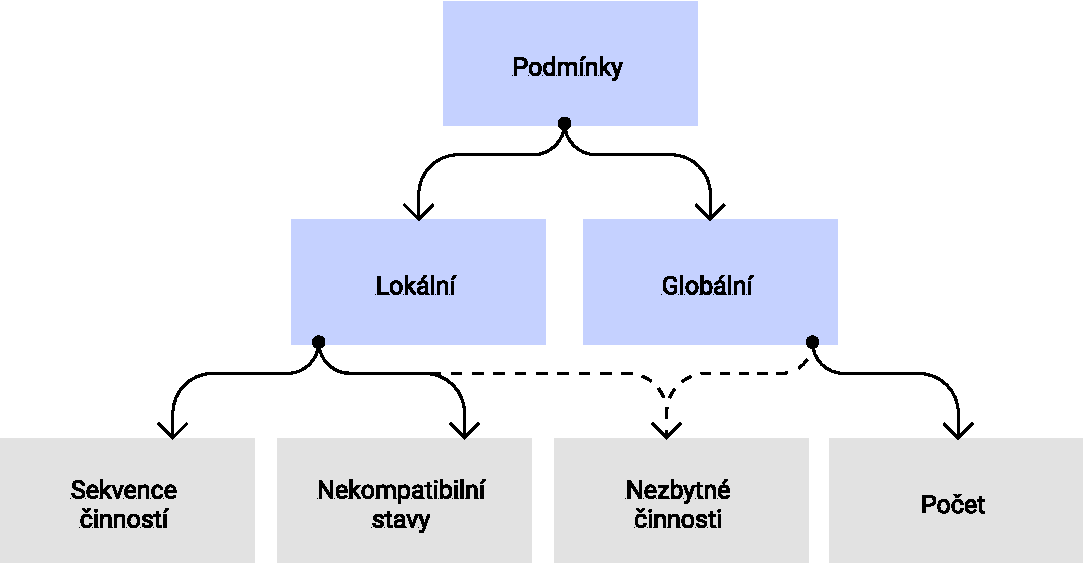
\includegraphics[scale=0.7]{img/constraints.pdf}
	\caption{Rozdělení podmínek dle jejich rozsahu}
	\label{fig:constraints}
\end{figure}

\section{Cílová funkce}
\label{sec:objective}
Cílová funkce je taková funkce, jejíž hodnotu je cílem optimalizovat (minimalizovat nebo maximalizovat). V~případě rozvrhování směn se může jednat o funkce vyjadřující rovnoměrnost obsazení směn, cenu, porušené zbytné podmínky \cite{blochliger2004modeling} či počet kontaktů mezi zaměstnanci (důležitý např. v~případě epidemie) \cite{zucchi2020personnel}.

Například v~případě optimalizace na základě vážených podmínek ji lze formulovat jako rov.~\ref{eq:objective}. Sankce za porušení nemusí být lineární, může jít i~o~konstantu, kvadratickou nebo libovolnou jinou funkci. \cite{kletzander2020solving}
\coloredeq{eq:objective}{
	f(\boldsymbol{x}) = \sum_{s = 1}^n c_s \cdot g_s(\boldsymbol{x}),
}
kde $\boldsymbol{x}$ je dané řešení, $n$ je počet zbytných podmínek, $c_s$ je váha~$s$-té~podmínky (také lze tento údaj chápat jako sankci za její porušení) a $g_s(\boldsymbol{x})$ je počet porušení $s$-té~podmínky v~řešení~$\boldsymbol{x}$. \cite{awadallah2015hybrid}

\section{Matematická interpretace řešení}
Řešení tohoto problému lze interpretovat jako trojrozměrnou binární matici $\boldsymbol{R}$, jejímiž parametry jsou zaměstnanec ($\forall i \in E$), den ($\forall j \in T$) a vypsaná směna ($\forall k \in S$), jednotlivé hodnoty $R_{ijk}$ jsou určeny funkcí \ref{eq:3dmatrix}. \cite{vaclavik2016roster} Takto má smysl řešení interpretovat pouze v~případě, že se obsazují striktně určené sloty pro směny.

\coloredeq{eq:3dmatrix}{
	R_{ijk} =
	\begin{cases}
		1, & \mbox{zaměstnanci $i$ je v den $j$ přiřazena směna $k$,} \\
		0, & \mbox{jinak.}\\
	\end{cases}
}


Příklad toho, jak lze řešení popsané ve funkci~\ref{eq:3dmatrix} interpretovat ve formě tabulky, je v~tab.~\ref{tab:interpretation}.
\begin{table}[h]
	\input{tables/interpretation-example.tex}
	\caption{Interpretace řešení}
	\label{tab:interpretation}
\end{table}


\section{Deterministické optimalizační metody}

Pro nalezení optimálního řešení mezi všemi možnostmi existuje celá řada metod~–~kromě vyčerpávajícího prohledání celého prostoru může jít o~matematické programování (lineární, kvadratické, nelineární, …).

\subsection{Lineární programování}

Úlohou lineárního programování je nalézt vektor $\boldsymbol{x}^{\ast} \in \mathbb{R}^n$ optimalizující hodnotu cílové funkce mezi všemi vektory, které splňují danou soustavu lineárních rovnic a nerovnic (kterým se zpravidla říká omezující podmínky nebo omezení). \cite{matousek2006linearni}

Celočíselné lineární programování je pro rozvrhování směn vhodné v jed\-no\-du\-chých případech, např.~když jsou pro všechny zaměstnance stanoveny stejné počty po sobě jdoucích pracovních dnů a volna a pro každý den je navíc stanoven minimální počet personálu a cílem je optimalizovat počet zaměstnanců tak, aby byla naplněna poptávka. \cite{satheeshkumar2014linear}

\subsection{Omezení deterministických optimalizačních metod}
Tyto metody obecně můhou přinést optimální výsledky, avšak pro reálné použití je jejich model příliš jednoduchý \cite{burke2004state}, případně špatně škálovatelný.

\section{Heuristika}

Většina stochastických metod vyskytujících se v~literatuře je rozšířením tzv.~metaheuristik, abstraktních metod pro řešení optimalizačních problémů, upravených na problém rozvrhování směn. Narozdíl od deterministických metod řešení není zaručeno, že bude nalezeno optimální řešení, cílem je získat výstup, který je dost dobrý, a to v~dostatečně krátkém čase (co konkrétně to znamená závisí na požadavcích). Neprobíhá tak vyčerpávající prohledávání všech kombinací. \cite{glover2015metaheuristics}

Metody se dají rozdělit do dvou základních skupin -- jedny iterativně rozšiřují částečné řešení, dokud není kompletně dokončeno (lokální vyhledávání), druhé pracují s~platným řešením, které iterativně vylepšují (vylepšovací metaheuristiky). \cite{van2013personnel}

\subsection{Výměna sousedících struktur}
Za účelem vytvoření nebo vylepšení rozvrhu je možné provádět řadu změn, dle \cite{kletzander2020solving} jde například~o:
\begin{itemize}
	\item přidání či odebrání směny,
	\item výměnu směny za jinou,
	\item změnu typu směny,
	\item změnu či vytvoření posloupnosti směn,
	\item výměnu směn mezi zaměstnanci,
	\item výměnu směn zaměstnance,
	\item zkrácení směny.
\end{itemize}


\subsection{Tabu search}
Základem tabu search je existence dvou druhů paměti – krátkodobé (obsahuje naposledy navštívená řešení) a dlouhodobé (obsahuje frekvenci návštěv). \cite{liang2020optimization} Vytváření a vylepšování řešení probíhá způsobem dle obr.~\ref{fig:tabusearch} tak, aby byly splněny podmínky. Prohledávání prostoru probíhá v~blízkém sousedství řešení, které je omezeno tak, aby se řešení nezacyklilo (jsou určeny zapovězené kroky -- tabu -- v~krátkodobé paměti, aby nebyla procházena stále stejná, dále již cílovou funkci nezlepšující řešení -- co je tabu, lze použít pouze tehdy, když řešení splňuje aspirační kritéria).  \cite{glover1990tabu}

\begin{figure}[h]
	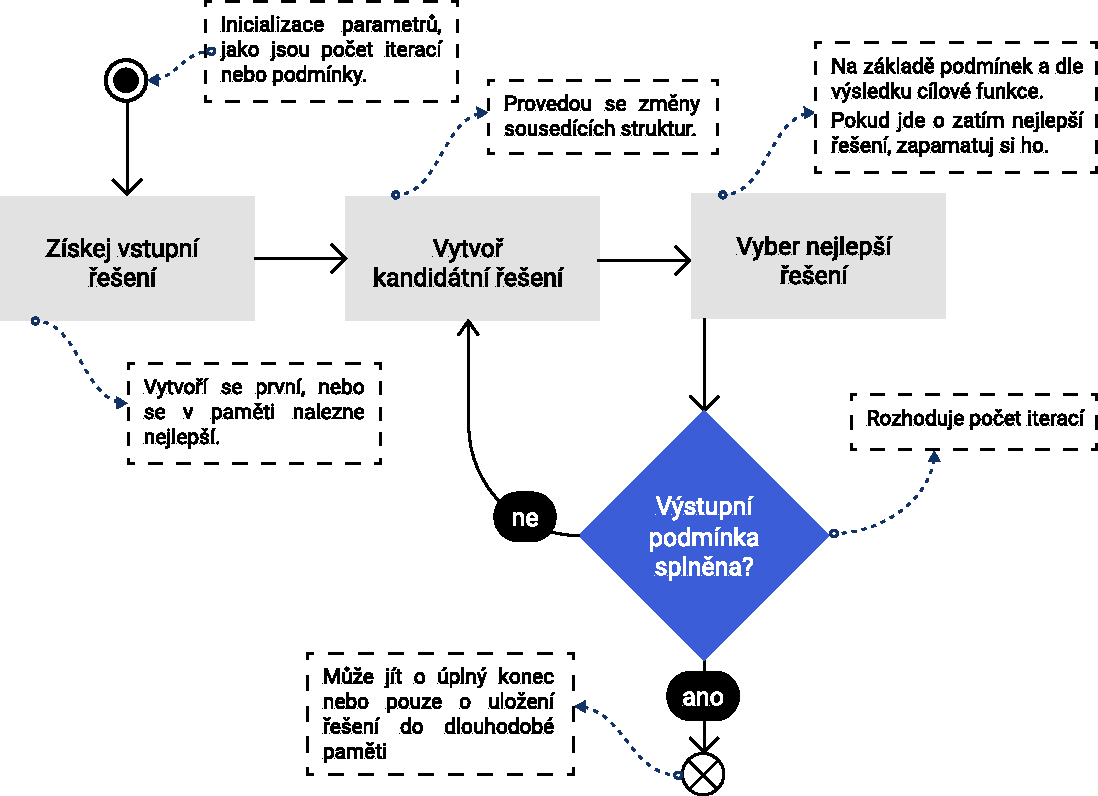
\includegraphics[scale=0.7]{img/tabu-search.pdf}
	\caption{Metaheuristika tabu search}
	\label{fig:tabusearch}
\end{figure}

 Algoritmus začíná inicializací řešení částečně náhodným způsobem tak, aby řešení neporušovalo nezbytné podmínky. Vylepšování referenčního řešení probíhá pomocí výměny sousedících struktur (dle podmínek např.~výměna posloupnosti směn mezi dvěma zaměstnanci). \cite{ramli2020tabu}

\subsection{Genetický algoritmus}

Genetický algoritmus je metaheuristika inspirovaná genetikou~--~používají se operace nazvané selekce chromozomů, křížení a mutace.

Narozdíl od tabu search se v~genetickém algoritmu prohledává větší množina řešení~–~začíná se s~počáteční populací řešení, v~níž se selektují nejlepší řešení, která se dále mezi sebou kříží~(kombinace náhodných částí), případně nahodile mutují. Algoritmus končí, pokud řešení konverguje~–~už se dlouhou dobu nepodařilo ho vylepšit. \cite{mallawaarachchi2017introduction}

Tento přístup lze aplikovat na rozvrhování směn například tak, že se jako chromozom kóduje kombinace dne, směny a zaměstnance. \cite{maenhout2011evolutionary}


\chapter{Analýza systému}

\section{Cílová skupina}
Aby bylo možné stanovit požadavky na aplikaci, byl vytvořen předpoklad o~cílové skupině pro tento systém. Jedná se o~menší firmu (případně malý tým v~rámci větší firmy) o~10 až 20 zaměstnancích, která podniká v~nekritickém vícesměnném provozu (např.~jedna pobočka řetězce rychlého občerstvení, restaurace nebo obchod). Firma zaměstnává jak pracovníky s~pracovní smlouvou, tak brigádníky na \acrshort{dpp}/\acrshort{dpc}. Vzhledem k~tomu řeší problém, jak rozvrhovat směny, stávající způsob je z~pohledu vedení firmy i samotných zaměstnanců neefektivní například z následujících důvodů:
\begin{itemize}
	\item brigádníci si musí směny domlouvat osobně,
	\item rozvrh je pověšen pouze na nástěnce,
	\item rozvrh se sestavuje manuálně,
	\item nedodržuje se týdenní pracovní doba,
	\item rozvrh je sestaven dle osobních preferencí vedoucího.
\end{itemize}


\section{Požadavky z~pohledu organizace}

Následující požadavky definují, jaké základní funkce by měl tento systém mít, a to především z~pohledu organizace, která by jej využívala (jedná se o~požadavky s~vysokou mírou abstrakce). Vychází se z~představy popsané výše, tedy že tento software je určen pro nasazení ve firmě, která momentálně není schopna efektivně připravovat rozvrhy směn a chtěla by ušetřit čas a zdroje, které na sestavení rozvrhu vynakládá.

\begin{enumerate}[label=\textbf{B\arabic*.}]
	\item Systém umožní distribuci rozvrhů směn k~zaměstnancům.
	\item Systém umožní zápis zaměstnance na~\acrshort{dpp}/\acrshort{dpc} na směnu.
	\item Systém vytvoří rozvrh směn na základě požadavků organizace.
	\item Systém bude automatizovat dohled nad dodržováním legislativy.
\end{enumerate}

\section{Doménový model}

V diagramu \ref{fig:domainmodel} je zadefinován předpokládaný doménový model firem cílové skupiny, jde o~znázornění skutečnosti, že ve firmě pracují zaměstnanci, kteří mají smlouvy a kterým jsou do jejich rozvrhu přiřazeny směny. Bližší popis doménového modelu je součástí přílohy \ref{app:analysis}.

\begin{figure}[h]
	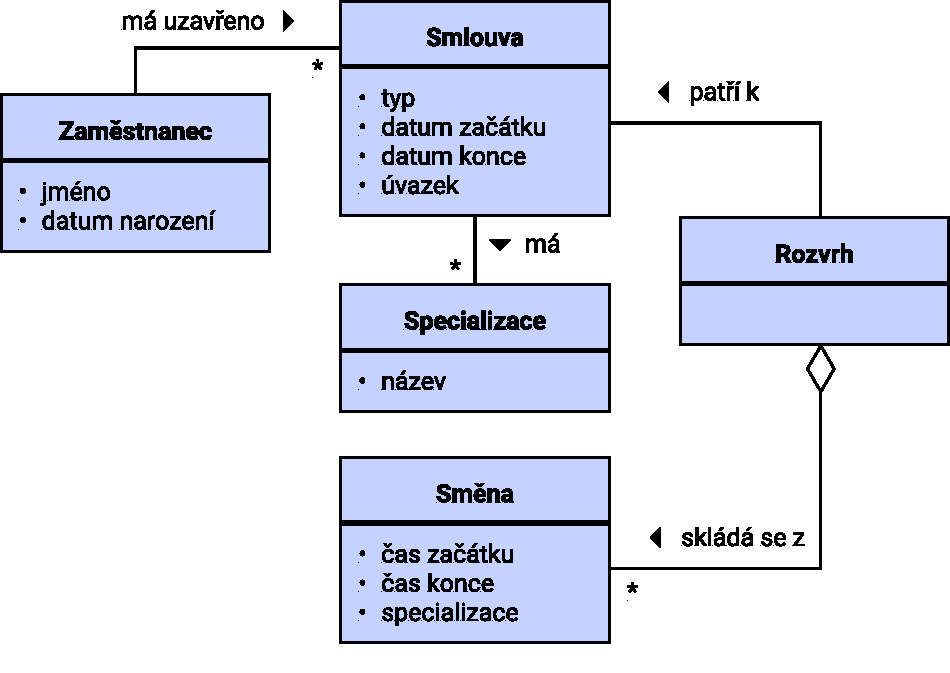
\includegraphics[scale=0.7]{img/domain-model.pdf}
	\caption{Doménový model}
	\label{fig:domainmodel}
\end{figure}

\section{Analýza existujících řešení}
\label{sec:existing}
Tato podkapitola bude věnována popisu již existujících nástrojů pro plánování lidských zdrojů. Jedná se o~komerční software, který byl otestován v~demoverzi, vzhledem k~tématu této práce byly hlavními sledovanými aspekty mobilní aplikace pro zaměstnance a~způsob rozvrhování směn.

Tyto systémy lze zařadit do kategorie tzv.~informačních systémů pro řízení lidských zdrojů, jejichž úkolem je obecně jak automatizovat, tak podporovat strategické rozhodování na základě dat. \cite{kovach2002administrative}

Byly vybrány informační systémy pro plánování lidských zdrojů, které alespoň částečně odpovídají uvedeným požadavkům z~pohledu organizací~–~podporují samoobslužné sestavování rozvrhů a případně i~tvorbu rozvrhů nějakým způsobem automatizují.

\subsection{Tamigo}
Aplikace Tamigo\footnote{\url{https://www.tamigo.cz/}} je komplexní aplikace pro plánování lidských zdrojů, je určena pro použití v~pohostinství, maloobchodě, zdravotnictví aj. \cite{tamigo2020reseni}

Aplikace je organizacím nabízena v~několika variantách, které jsou zpop\-lat\-ně\-ny podle množství podporovaných funkcí (jedná se např. o~rozpisy směn všech zaměstnanců, výkazy práce, správu absencí, správu mezd smluv zaměstnanců, evidenci příchodů a odchodů) a počtu zapojených zaměstnanců. Mezi součásti tohoto produktu patří webové rozhraní i mobilní aplikace (přestože jde o nativní aplikaci, v~testované verzi funguje pouze v~případě, že je uživatel online, jinak padá). Uživatelské role jsou v~tomto systému Administrátor, Manažer a Zaměstnanec.

Systém umožňuje manažerům vytvářet rozvrh, částečně je tento proces manuální, částečně lze rozvrh vygenerovat na základě šablon, které si uživatel předem připraví (např. obvyklá pracovní doba pro jednotlivé zaměstnance).

Za\-měst\-na\-nec si může aktualizovat osobní data, zobrazit osobní rozvrh směn, žádat o dovolenou a sledovat stav jejího čerpání, zobrazit výkaz práce pro výplatní období, aj.

\subsection{Tanda}
Na podobném principu jako aplikace Tamigo pracuje i~aplikace Tanda\footnote{\url{https://www.tanda.co/}}. Automatické rozvrhování funguje na principu šablon -- rozvrh se tedy vytvoří jednou a následně se opětovně používá \cite{tanda2020rosters}.

I tento systém má jak webové, tak mobilní rozhraní, obojí pro zaměstnance i vedoucí. Mobilní rozhraní opět nepodporuje ani čtení dat v~případě, že je uživatel offline.

\subsection{When I Work}
Aplikace When I Work\footnote{\url{https://wheniwork.com}} má opět webové i mobilní rozhraní. Rozvrhování zde opět funguje manuálně nebo na základě šablon, aplikace v~placené Pro verzi \cite{wheinwork2020pricing} však podporuje i automatické přiřazení volných směn k~vhodným zaměstnancům (v~potaz při rozvrhování bere pracovní pozici, již existující směny, požadavky na volno a další filtry). \cite{wheinwork2020employee} Mobilní aplikace umožňuje zaměstnancům zadat, jakou pracovní dobu preferují nebo kdy jsou naopak nedostupní. Ani tato aplikace nefunguje v~offline režimu.

\subsection{Shrnutí}
Vyzkoušené informační systémy se v~principu příliš neliší a nabízejí podobné základní prvky (mobilní a webové rozhraní; uživatelské role; komplexní správa mezd, docházky, rozvrhů). Společné mají i to, že žádná z~aplikací neimplementuje ani částečný offline režim, což může být pro uživatele v~některých situacích nepříjemné (lze ale předpokládat, že mobilní aplikace nebyla tvůrci považována za prioritní v~porovnání s~webovým rozhraním). Liší se však způsobem, jakým rozvrhují směny -- největší automatizaci zde poskytuje aplikace When I Work. Dalším rozdílem je uživatelská přívětivost, její hodnocení by však bylo spíše subjektivní.

Alternativou systémů, které přímo odpovídají požadavkům, mohou být komplexnější \acrshort{erp} systémy a jejich modul pro plánování lidských zdrojů.

\section{Požadavky na systém}
Na základě požadavků ze strany organizace a~po otestování podobných aplikací byly stanoveny požadavky na funkce nového systému, které byly rozděleny do několika kategorií podle cílového uživatele. Při implementaci systému na plánování směn je žádoucí, aby byl dohled nad dodržováním pracovněprávních předpisů (především těch, které uvádějí kvantitativní údaje), automatizován, proto jsou rovněž uvedeny požadavky vyplývající z~analýzy legislativy (viz podkapitolu \ref{section:legislativa}).

\subsection{Uživatelé}
\begin{enumerate}[label=\textbf{U\arabic*.}]
		\item Systém bude personalizovaný podle potřeb daného uživatele.
\end{enumerate}

\subsection{Zaměstnanci}
\begin{enumerate}[label=\textbf{Z\arabic*.}]
		\item Systém umožní zaměstnancům náhled do jejich rozvrhu.
		\item Systém umožní zaměstnancům na \acrshort{dpp}/\acrshort{dpc} zápis na směnu.
\end{enumerate}

\subsection{Organizace}
\begin{enumerate}[label=\textbf{O\arabic*.}]
	\item Systém umožní registraci nových organizací.
	\item Systém umožní přidávání nových zaměstnanců.
	\item Systém umožní automatické přiřazení směn.
	\item Systém umožní plánování směn na následující týdny.
	\item Systém umožní náhled na rozvrh zaměstnanců.
\end{enumerate}

\subsection{Legislativa}
\begin{enumerate}[label=\textbf{L\arabic*.}]
		\item Systém umožní náhled do osobního rozvrhu nejméně 2 týdny předem.
		\item Systém umožní zaměstnancům na dohodu o~provedení práce odpracovat nejvýše 300~hodin v~kalendářním roce.
		\item Systém umožní zaměstnancům na dohodu o~pracovní činnosti odpracovat nejvýše 20~hodin týdně v~průměru 52 týdnů.
		\item Systém rozvrhne směny s~ohledem na 40hodinovou týdenní pracovní dobu a úvazky jednotlivých zaměstnanců.
\end{enumerate}

\section{Aktéři, uživatelské role}
Jedním z~hlavních cílů systému na plánování směn je informovat každého zaměstnance o jeho směnách, proto se jeví vhodnou personalizace, které se docílí s~pomocí uživatelských účtů. Vstupní operací bude přihlášení -- z~toho vyplývá nezbytnost existence role přihlášeného a nepřihlášeného uživatele.

Roli přihlášeného uživatele je nutné dále rozšířit, konkrétně na zaměstnance a roli, kterou má v~rámci tohoto systému osoba, která má zodpovědnost za rozvrhování pracovní doby (vedoucí) a která by měla mít komplexní přehled o~rozpisu i možnost do něj zasáhnout.

Jednotliví zaměstnanci pak v~systému mohou být různými aktéry, především na základě pracovněprávního vztahu (tj. zaměstnanec v pracovním poměru, zaměstnanec na dohodu o provedení práce a zaměstnanec na dohodu o pracovní činnosti), viz obr.~\ref{fig:userroles}. Důvodem je, že aktéři budou moci provádět specifické operace a systém s~nimi bude interagovat odlišně. Rozhodujícím faktorem není to, zda má zaměstnanec plný nebo zkrácený úvazek, v obou případech platí stejné podmínky a liší se jen týdenní pracovní doba, stejně tak nezáleží na tom, zda je zaměstnanec nezletilý.

\begin{figure}[h]
	\input{img/actors.pdf_tex}
	\caption{Diagram aktérů}
	\label{fig:userroles}
\end{figure}

\newpage
\section{Uživatelské příběhy}\label{uc-analysis}

Pro analýzu systému z~pohledu uživatelské interakce byl zvolen neformální způsob inspirovaný uživatelskými příběhy (user stories), hlavní výhodou je využití běžného jazyka. Přehled uživatelských příběhu ve zjednodušené podobě je na obr.~\ref{fig:user-stories}, jejich podrobnější mapa je součástí přílohy \ref{app:analysis}. Součástí přílohy~2 jsou i nákresy uživatelského rozhraní včetně popisu, viz~obr.~\ref{fig:lfp}


\begin{figure}[h!]
	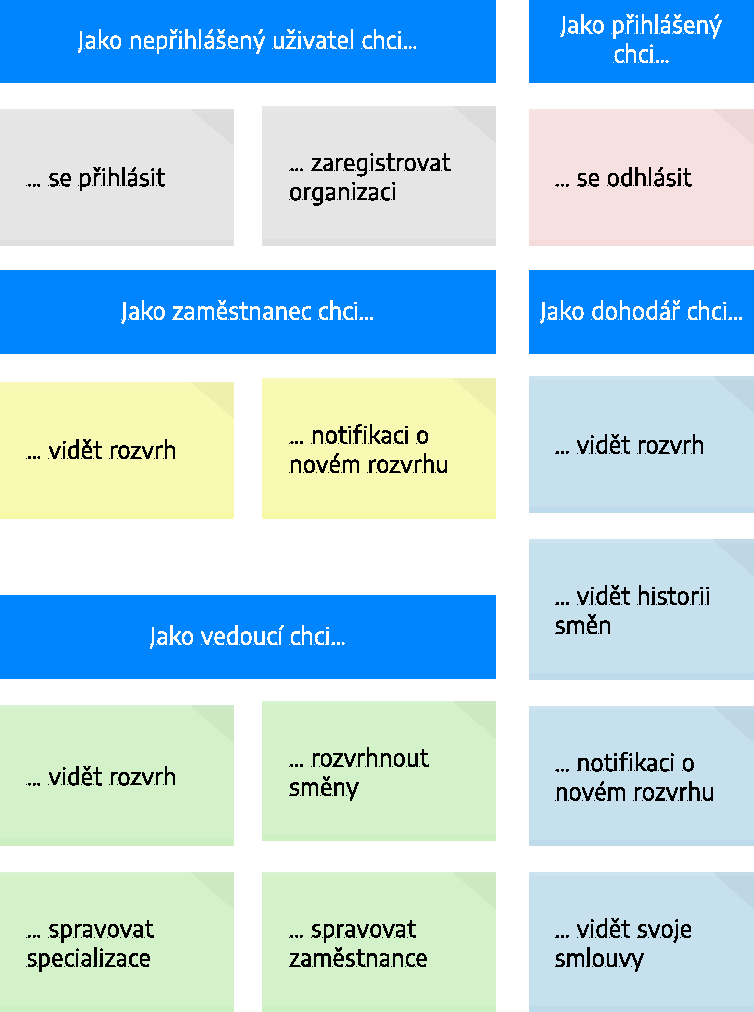
\includegraphics[scale=0.7]{user-stories.pdf}
	\caption{Zjednodušený přehled uživatelských příběhů}
	\label{fig:user-stories}
\end{figure}

\begin{figure}
	\begin{subfigure}{\textwidth}
		\centering
		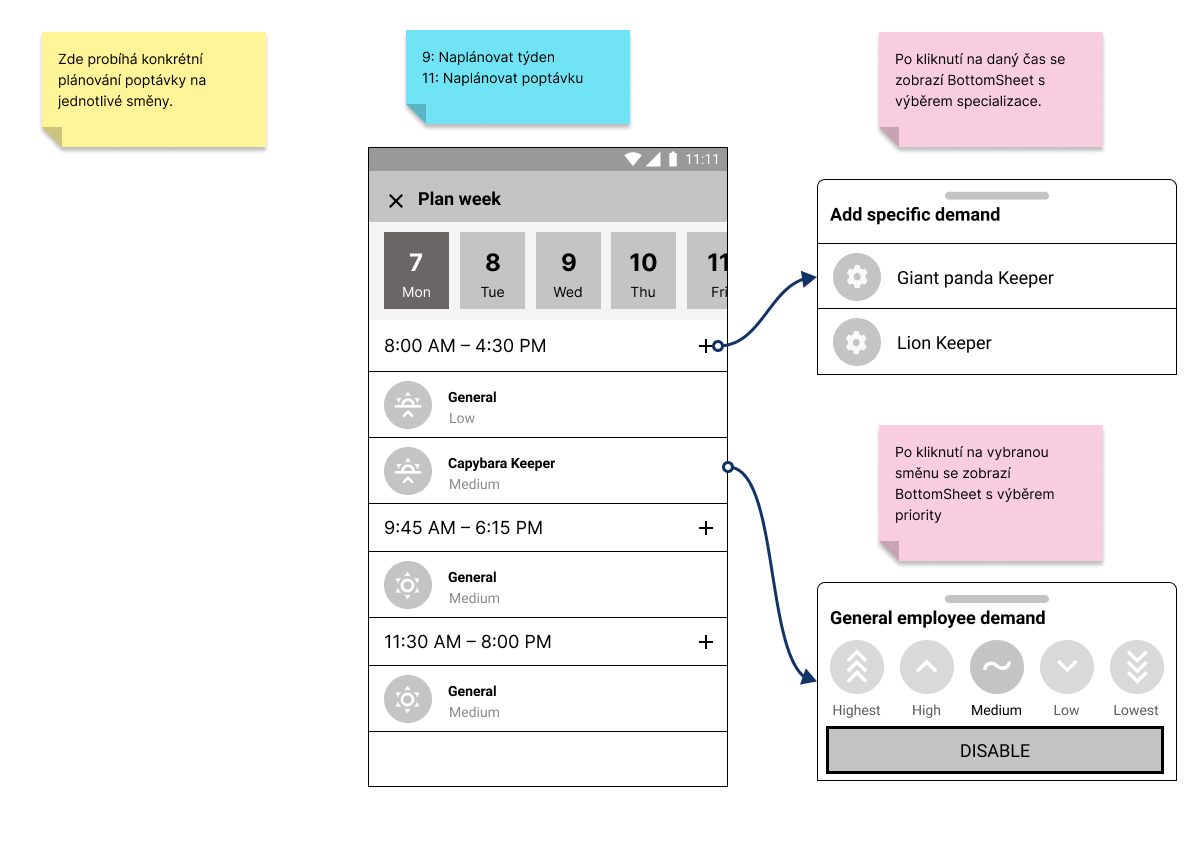
\includegraphics[width=\textwidth]{Demand.png}
		\caption{Obrazovka pro úpravu poptávky}
		\label{sub:lfp1}
	\end{subfigure}

	\begin{subfigure}{\textwidth}
		\centering
		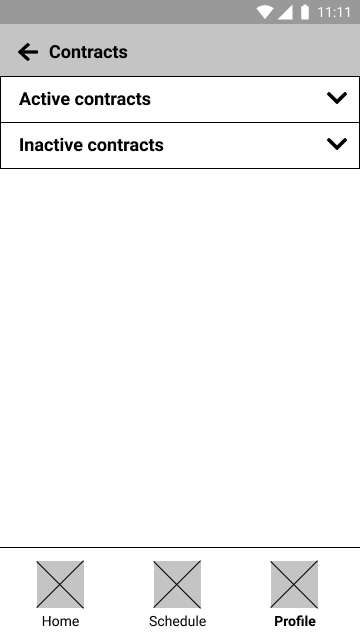
\includegraphics[width=\textwidth]{contracts.png}
		\caption{Obrazovka se seznamem smluv}
		\label{sub:lfp2}
	\end{subfigure}

	\caption{Ukázka nákresů UI}
	\label{fig:lfp}
\end{figure}


\newpage

\part{Praktická část, implementace}

\chapter{Výběr technologií}

\section{Technologie pro uživatelské rozhraní}

V~případě, že by byla aplikace určena k~nasazení v~produkčním prostředí, připadaly by v~úvahu nejméně dva přístupy -- mobilní nebo webová aplikace.

\begin{figure}[h!]
	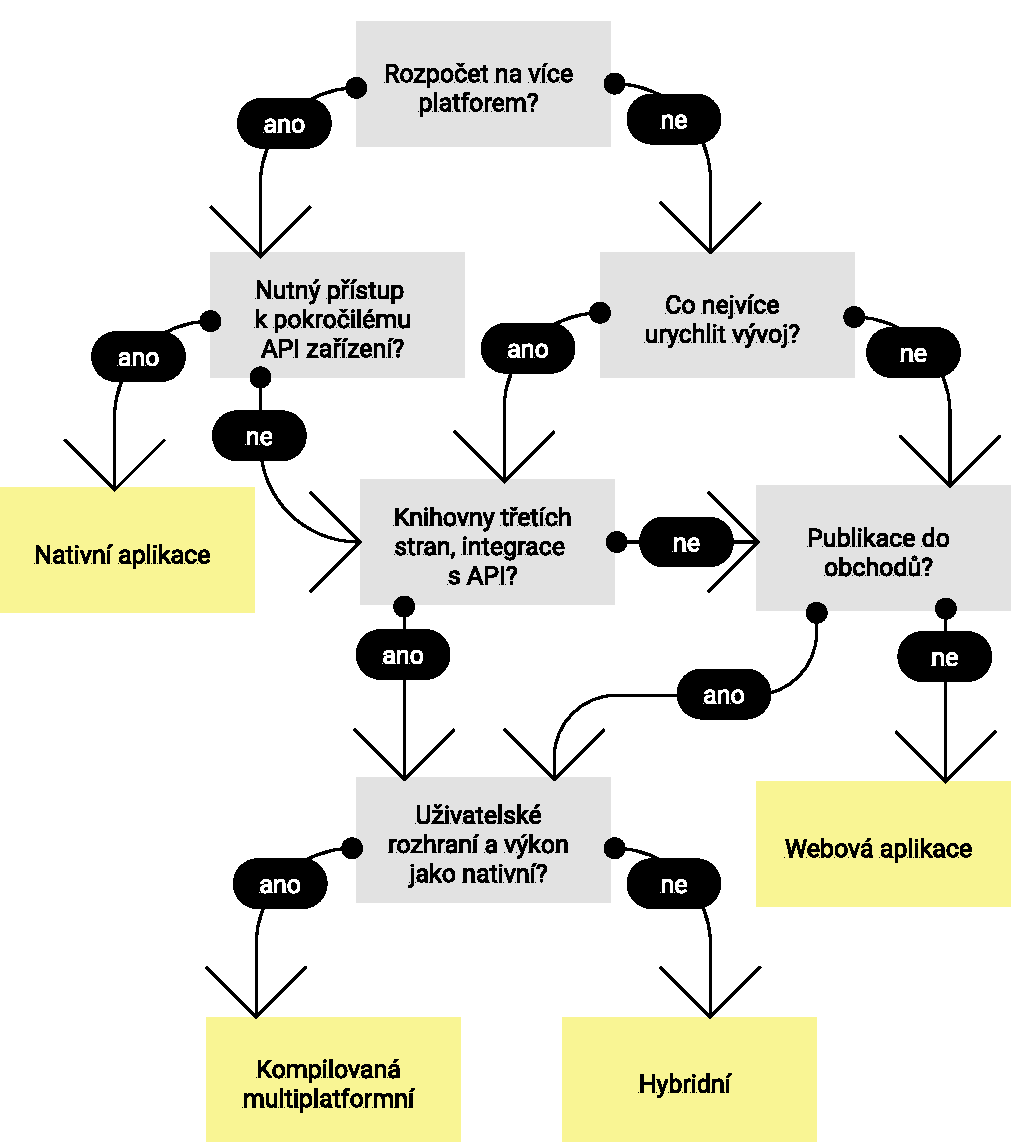
\includegraphics[scale=0.7]{img/app-decision-tree.pdf}
	\caption{Rozhodovací strom pro vývoj na mobilní zařízení}
	\label{appdecisiontree}
\end{figure}

\subsection{Webová aplikace}
Pro použití webové aplikace hovoří fakt, že je není třeba žádným způsobem instalovat a stačí prosté zadání adresy do internetového prohlížeče, z~podstaty věci je multiplatformní, lze ji zobrazit jak na počítači, tak na mobilním zařízení, jedná-li se o responzivní aplikaci, může být i~její použití na mobilním zařízení uživatelsky přívětivé. Nevýhodami jsou omezené možnosti při implementace offline režimu, i to, že z hlediska rychlosti se nativním mobilním aplikacím nevyrovnají. \cite{stevens2018what}

\subsection{Mobilní aplikace}

Vyplývá-li podpora mobilní platformy z~požadavků, ilustruje další rozhodování o~způsobu implementace strom na obrázku \ref{appdecisiontree} (vychází z~\cite{matyunina2020native}), především ale záleží na prioritách toho, kdo danou aplikaci chce uvádět na trh.

Oproti responzivnímu webu mají nativní aplikace výhodu, že mohou jednoduše přistupovat k \acrshort{api}, které poskytuje zařízení, na kterém jsou nainstalované, tedy mohou snadno získat přístup k fotoaparátu či poloze zařízení; také lze na zařízení jednoduše přijímat notifikace, i když je aplikace na pozadí. Nativní aplikace mohou být vhodné i pro použití v offline režimu, aplikace může mít lokální databázi.

Nevýhodou pro uživatele je, že se musí instalovat na zařízení. S~tím souvisí i o~něco složitější způsob distribuce -- v~případě, že je možné zveřejnit aplikaci v~obchodech (Google Play, AppStore), musí projít schvalovacím procesem, což může trvat několik dní a nemusí být vždy úspěšné, např. v~případě, že aplikace obsahuje nevhodný obsah, narušuje něčí autorská práva nebo nevhodným způsobem zpracovává osobní údaje uživatelů. Je třeba uvádět, jaká oprávnění pro přístup ke mobilním \acrshort{api} (SMS, kontakty, poloha, soubory, aj.) aplikace požaduje. \cite{google2021policy}.

Při výběru konkrétního způsobu implementace mobilní aplikace pak existuje několik dalších rozhodovacích situací, především~výběr podporované platformy.

\subsubsection{Platforma}
Na trhu s~chytrými mobilními zařízeními jsou dvě dominantní platformy, Android (podíl na trhu celosvětově 72~\%) a iOS (podíl na trhu 27,5~\%) \cite{statcounter2021mobile}. Nevýhodou rozšířenějšího Androidu oproti iOS je fragmentace, tzn. existence velké řady různých zařízení, která je třeba podporovat. Pro účely této práce bude podporována pouze platforma Android.


\subsubsection{Způsob vývoje}

Je-li nezbytné podporovat více platforem, je možné vyvinout aplikaci multiplatformně, hybridně, případně pro každou platformu zvlášť.

\paragraph{Multiplatformní vývoj}
Multiplatformní vývoj umožňuje nasazení jedné aplikace na více platformách, kód pro všechny platformy je sdílený, jádro aplikace tedy není třeba duplikovat, což je jejich nespornou výhodou, navíc to může i snížit náklady na vývoj.

Problémem je přístup k~aplikačnímu rozhraní a hardwaru daného zařízení, omezené možnosti při používání knihoven specifických pro platformu nebo složitější vývoj uživatelského rozhraní tak, aby odpovídalo konvencím pro všechny platformy. \cite{manchanda2020where}   Používají se frameworky jako Flutter (jazyk Dart), React Native (JavaScript) nebo Xamarin (C\#).

\paragraph{Vývoj pro danou platformu}
V~případě vývoje na jednu platformu je možné používat všechny součásti zařízení naplno. Co se přístupu k hardwaru, výkonu a uživatelské přívětivosti týče, mají nativní aplikace nad multiplatformními jasnou převahu, jejich vývoj je však dražší. \cite{dennis2018native}

\paragraph{Hybridní vývoj}
Hybridní aplikace jsou kombinací webu a nativní mobilní aplikace – použijí se standardní technologie pro vývoj webu (\acrshort{html} + \acrshort{css} + JavaScript), toto se obalí do nativní aplikace, v~níž běží webový prohlížeč. Jejich největší výhodou je cena, rychlost vývoje a jednodušší správa. Stinnou stránkou tohoto přístupu je menší uživatelská přívětivost, omezený přístup k~\acrshort{api} zařízení nebo nižší výkon v~porovnání s~plně nativní aplikací. \cite{design2020ultimate}


\subsubsection{Programovací jazyk}
Pro nativní vývoj na platformu Android lze vybrat nejméně ze tří možností, a to C/C++, Javy a Kotlinu. Toto rozhodování může v~této době u~nových projektů probíhat spíše pouze v teoretické rovině, neboť oficiální podporu ze strany Googlu má nejmodernější jazyk Kotlin.

Mezi hlavní výhody Kotlinu oproti jiným variantám patří null-safety (bezpečné volání na objektech, které mohou nabývat hodnotu \texttt{null}), coroutines (odlehčená verze vláken pro asynchronní operace) nebo Kotlin Extensions (knihovny nejrůznějších funkcí usnadňující vývoj obecně i specificky pro Android). \cite{android2021kotlin}

Obdobné rozhodování může probíhat i~v~případě platformy iOS, pro kterou se nabízí použití Swiftu nebo starého jazyka Objective-C. Ze strany Applu je doporučena modernější varianta (Swift), protože aplikace jsou rychlejší a vývoj snazší.

\subsubsection{Architektonický vzor}
Standardním architektonickým vzorem používaným při vývoji Android aplikací je \acrshort{mvvm}. \cite{android2020guide}. Aplikace má tři vrstvy, které spolu komunikují způsobem naznačeným na obr.~\ref{fig:mvvm}. Hlavním cílem je oddělit prezentační vrstvu od business logiky.  \cite{shekhar2020mvvm}

\begin{figure}[h!]
	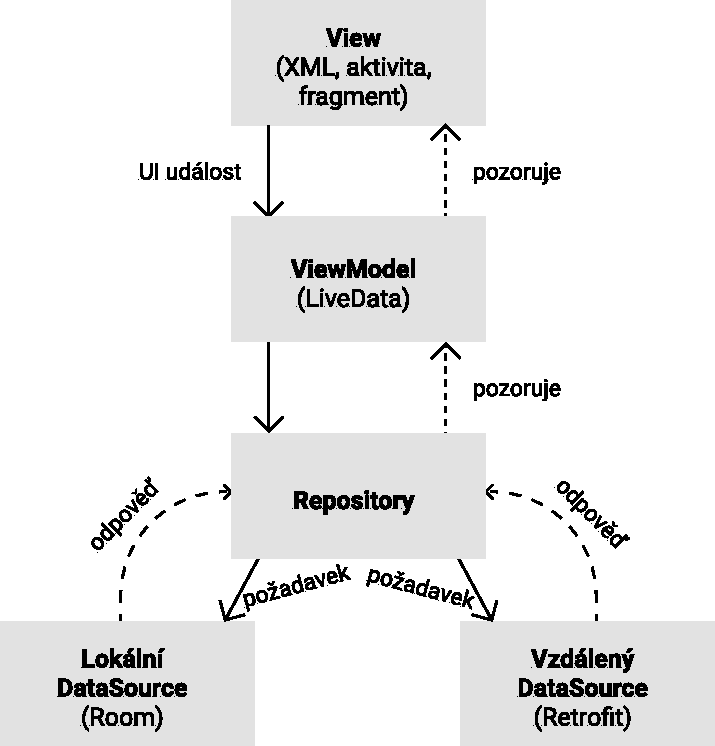
\includegraphics[scale=0.7]{img/mvvm-architecture.pdf}
	\caption{Komunikace mezi vrstvami v~\acrshort{mvvm}}
	\label{fig:mvvm}
\end{figure}

\acrshort{mvvm} vychází ze staršího architektonického vzoru \acrshort{mvp}, Presenter je podobný jako ViewModel, hlavním rozdílem je, že Presenter si drží referenci na View (relace mezi View a Presenterem je 1:1) a řídí, kdy se má View aktualizovat, kdežto ViewModel neví, jaký View ho pozoruje a relace mezi View a ViewModelem je 1:$n$. \cite{vogel2017android} Nadstavbou nad \acrshort{mvvm} je tzv.~Clean Architecture, která zaručuje ještě větší oddělení prezentační vrstvy a business logiky (Android aplikace se rozděluje do více modulů, nejčastěji nazvaných Presentation, Domain a Data). \cite{jain2019kotlin}

Vzhledem k~předpokládané velikosti projektu byl zvolen doporučený architektonický vzor \acrshort{mvvm}.

\subsection{Shrnutí}

Jako nejvhodnější by se v~případě produkčního nasazení této aplikace jevilo zkombinovat dva přístupy, tedy mít uživatelské rozhraní jak ve formě webové aplikaci, tak mít i podpůrnou mobilní aplikaci. Tento přístup byl také zvolen v případě většiny podobných řešení (viz podkapitolu \ref{sec:existing}). Zde bude implementována pouze jedna část, a to mobilní aplikace, neboť důraz bude kladen především na pohodlí zaměstnanců, kteří chtějí mít svůj rozvrh po ruce co nejrychleji.

Mobilní aplikace bude vyvinuta jako nativní Android aplikace, v~produkčním prostředí by bylo žádoucí uživatele iOS nediskriminovat, a aplikaci jim také nabídnout, z~tohoto důvodu by bylo vhodné zvážit použití nějakého multiplatformního frameworku, rozhodující by byly plány na budoucí vývoj, případně i~finance. Pro vývoj se použije programovací jazyk Kotlin, protože se jedná o moderní programovací jazyk, který je pro vývoj na danou platformu nejvhodnější. Aplikace bude navržena dle zásad architektonického vzoru Model-View-ViewModel.


\section{Backendová technologie}

\subsection{Webový framework}

Webové frameworky, tj. knihovny zdrojových kódů připravené pro tvorbu webů (především jejich serverové strany), se standardně používají pro zjednodušení vývoje a nasazení aplikací. Ať už jsou napsány v~libovolném programovacím jazyce (může jít např.~o~PHP, Javu, Ruby nebo Python), standardními součástmi jsou perzistence dat, autentizace uživatelů, správa session nebo šablony pro uživatelské rozhraní. Společnou mají také podporu pro architektonický vzor \acrshort{mvc}. \cite{docforge2014web}

Z~množství variant, které se nabízejí, byl zvolen framework Ruby on Rails (v~jazyce Ruby), a to především z~důvodu jeho filosofie Don't Repeat Yourself (kód by měl být znovupoužitelný, bez zbytečného opakování) a Convention Over Configuration (webová aplikace je nakonfigurována dle konvencí, a vývojář tak nemusí trávit čas psaním konfiguračních souborů) \cite{rails2020}, která slibuje výrazné usnadnění vývoje.

\subsection{Aplikační rozhraní}

Pro komunikaci s~dalšími aplikacemi (zde především pro komunikaci klienta se serverem) musí aplikace vnějšku poskytnout své aplikační rozhraní. Za tímto účelem existuje několik možností, které jsou vhodné pro různé případy (např.~\acrshort{rest}, SOAP, GraphQL, gRPC). Tyto způsoby implementace se mohou od sebe odlišovat formátem přenosu (binární, textový) nebo protokolem (\acrshort{http} i~jiné).

Pro účely tohoto projektu se jako optimální varianta jeví použití \acrshort{rest} \acrshort{api}, a to vzhledem k~velmi dobré podpoře ze strany webového frameworku bez nutnosti rozšiřování o~další knihovny. %(konkrétně Ruby on Rails podporují vytváření cest na základě konvencí – pokud tak controller definuje metodu \texttt{update}, automaticky se vytvoří endpoint \texttt{PUT/PATCH /resources/:id}, případně lze cesty definovat v~souboru \texttt{config/routes.rb} a provolat tak libovolnou akci v~libovolném controlleru).

V některých případech by bylo vhodnější použít pro komunikaci jiný prostředek (především v~případě volání výpočtů na serveru), např.~\acrshort{rpc} (gRPC, \acrshort{xml}-\acrshort{rpc}, \acrshort{json}-\acrshort{rpc} či jinou konkrétní implementaci), neboť zde nedochází k~přenosu zdrojů, ale pouze k~výpočtům na vzdáleném serveru (provolávání akcí). \cite{sturgeon2016understanding} Toto by ale vytvořilo problémy při nasazení aplikace na \acrshort{paas} službách (např. Heroku) \cite{lisitsky2018does}, proto bylo zvoleno řešení, které sice není z~hlediska architektury tou nejlepší volbou, ale jeho  použití je flexibilnější.

\subsection{Databáze}

Rozhodování ohledně použité databáze se může týkat způsobu uložení dat (relační nebo No\acrshort{sql}) a samotného \acrshort{dbms} (systém správy báze dat). Je třeba se rozhodnout, zda v~projektu bude použita relační či No\acrshort{sql} databáze. Relační databáze přitom jsou vhodné na ukládání dat se statickou strukturou, No\acrshort{sql} databáze mohou být flexibilnější, co se ukládání dat týče.  \cite{geeks2020difference}

Pro účely tohoto projektu byla zvolena relační databáze, a to z~důvodu předem určené struktury dat a taktéž proto, že jde o technologii, která má dobrou podporu, a to i ze strany webových frameworků. Upřednostněna tedy byla tradiční technologie. Jako konkrétní \acrshort{dbms} byl zvolen Postgres.


\subsection{Shrnutí}

Aplikace bude vyvinuta ve webovém frameworku Ruby on Rails, a to vzhledem k~tomu, že jde o~rozšířený framework, který slibuje jednoduchou konfiguraci. Z~volby frameworku vyplývá použit architektonického vzoru \acrshort{mvc}. S~vnějškem bude tato aplikace komunikovat prostřednictvím \acrshort{rest} \acrshort{api} vzhledem k~jednoduché implementaci a silné podpoře pro jeho využití. Použita bude relační databáze, konkrétně Postgres.

\section{Požadavky na kvalitu software}

Z~rozhodování v~této kapitole vyplynuly následující požadavky na kvalitu software:

\begin{enumerate}[label=\textbf{S\arabic*.}]
	\item Bude vyvinuta nativní Android aplikace v~jazyce Kotlin.
	\item Backend bude vyvinut ve webovém frameworku Ruby on Rails.
	\item Mobilní aplikace bude se serverem komunikovat přes jeho \acrshort{rest} \acrshort{api}.
	\item Bude použita databáze Postgres.
\end{enumerate}

\chapter{Návrh vlastního algoritmu}

\section{Požadavky na rozvrh}

Z~hlediska klasifikace uvedené v~podkapitole~\ref{sec:clasif} půjde o neperiodický rozvrh s~flexibilními parametry, cílem bude spíše rozhodnout než řešení co nejvíce optimalizovat.

Nezbytné podmínky budou dány legislativními požadavky na rozvrh směn, rozvrh bude sestaven na týden, cílem je netvořit zbytečné překážky v~zaměstnání a rozvrhnout práci všem zaměstnancům, kterým nebudou směny rozvrženy jiným způsobem (manuálně vedoucím nebo samostatně zaměstnancem). Zbytné podmínky byly vybrány dle možných manažerských požadavků na rozvrh směn.

Konkrétní požadavky byly stanoveny následovně:
\begin{enumerate}
	\item Algoritmus rozvrhne směny na jeden týden.
	\item Algoritmus rozvrhne směny v~celém dni na základě poptávky.
	\item Algoritmus rozdělí směny mezi zaměstnance v~pracovním poměru.
	\item Algoritmus vezme v~potaz legislativní požadavky (přestávka, úvazek, maximální délka směny).
\end{enumerate}

\section{Tvorba směn a poptávky}\label{sub:demand}
Při rozvrhování se pro zjednodušení předpokládá, že v každém týdnu budou vypsány směny pravidelným způsobem, to znamená, že všechny budou stejně dlouhé a budou každý den v~týdnu začínat ve stejnou dobu, a budou v rámci jednoho pracovního dne rozloženy pravidelně dle počtu směn (pro realističtější modelování situace existuje možnost některé směny z rozvrhu vyjmout). Půjde tak flexibilně stanovit parametry rozvrhování, konkrétně celkovou pracovní dobu, délku jedné směny, délku přestávky a počet směn v jednom dni. Bude také možné naplánovat směny probíhající přes noc, případně i~24hodinový provoz (pak bude třeba stanovit začátek jedné ze směn, aby bylo možné jejich rovnoměrné rozdělení). Pro každou jednotlivou směnu lze dále určit její prioritu (číslo mezi 0~a~5 určující, zda má směna být rozvržena více nebo méně zaměstnancům vzhledem k~celku).

\section{Podmínky}
Obdobně jako v~podkapitole \ref{sec:constraints} se podmínky dají rozdělit do dvou skupin (nezbytné a zbytné) tak, že při porušení nezbytných podmínek vůbec nebude rozvrh možné uložit do databáze (lze určovat, zda je řešení validní či nikoli), zbytné podmínky budou pouze \uv{doplňkem}, který říká, jak moc je dané řešení kvalitní z~hlediska požadavků, které si klade manažer.

\subsection{Nezbytné podmínky}
Pro určení nezbytných podmínek byly využity poznatky z~oblasti legislativy (viz podkapitolu \ref{section:legislativa}), především maximální délka směny, minimální přestávka mezi koncem jedné směny a začátkem další, týdenní pracovní doba, dále také určení specializace.

Rozvhování probíhá v~transakci a tyto podmínky jsou vyhodnocovány na úrovni modelů, v~případě, že budou porušeny, bude vyvolána výjimka, dojde k~rollbacku a zahození celého rozvrhu.

Konkrétně se jedná o následující podmínky:

\begin{enumerate}
	\item Zaměstnanec v~celém týdnu odpracuje nejvýše počet hodin úměrný svému úvazku.
	\item Mezi koncem jedné směny a začátkem další bude nejméně 12hodinová přestávka.
	\item Zaměstnanec může být přiřazen pouze na směnu, která nemá žádnou specializaci nebo má stejnou specializaci jako zaměstnanec.
	\item Zaměstnanec může být v jednu chvíli pouze na jedné směně, směny se nesmějí překrývat.
\end{enumerate}

\subsection{Zbytné podmínky a cílová funkce}
Byly zvoleny čtyři zbytné podmínky (obsazení všech směn, obsazení směn úměrně poptávce, obsazení specializovaných směn, více volna v~kuse), podle kterých bude možné určovat, jak moc je dané validní řešení kvalitní. Pro každou z~nich byl zvolen způsob, jak se bude počítat cílová funkce, dále byl stanoven pokud možno co nejjednodušší způsob, jak optimalizovat hodnotu cílové funkce. Váhy jednotlivých kritérií se určují při volání algoritmu, pokud je váha nulová, daná strategie pro vylepšování rozvrhu neproběhne.

Cílová funkce je stanovena obdobně jako v~podkapitole \ref{sec:objective} – jde o~součet vážených porušení zbytných podmínek (sankce za porušení je lineární).

\subsection{Obsazení všech směn}

Smyslem této podmínky je určit, zda v~každou chvíli bude na pracovišti alespoň jeden zaměstnanec. Vyhodnocení probíhá tak, že se naleznou všechny směny, které nemá do svého rozvrhu zapsán žádný zaměstnanec. Výsledkem cílové funkce je počet neobsazených směn násobený sankcí.

\subsection{Obsazení směn úměrně poptávce}
Jak již bylo uvedeno v podkapitole \ref{sub:demand}, každá ze směn může mít určenou svou prioritu v~závislosti na tom, jak moc velké množství zaměstnanců je v~daném čase na pracovišti potřeba. Penalizována je odchylka od požadovaného obsazení $\texttt{D[i]}$ pro $\texttt{i} = \mbox{priorita dané směny}$ v~souhrnném rozvrhu (jde tak o~globální podmínku).


\subsubsection{Rozložení poptávky}
Pro účely rozložení poptávky mezi směny s~různou prioritou byl navržen následující postup: nejprve se spočítá průměrná priorita (\texttt{avg\_priority}) ze všech směn v~daném období a průměrný počet zaměstnanců na jednu směnu (\texttt{avg\_assignments}, počet přiřazení na směnu dělený počtem směn).

Z těchto údajů se vypočítá požadovaný počet zaměstnanců na směně o~střední prioritě (\texttt{medium\_demand = 3}). \texttt{const} je nějaká konstanta, která ovlivňuje rozložení poptávky (viz tab.~\ref{tab:demandfactor}). Hodnota konstanty by měla být alespoň \texttt{medium\_demand}, aby poptávka byla kladné číslo. S~výsledkem rov.~\ref{eq:d3} a \ref{eq:di} se pracuje v zaokrouhlené formě (může tak docházet k~chybě).

\begin{equation}
	\label{eq:d3}
	\texttt{D[3]} = \texttt{avg\_assignments} \cdot \frac{\texttt{1 + (3 - avg\_priority})}{\texttt{const}}
\end{equation}

\begin{equation}
	\label{eq:di}
	\texttt{D[i]} = \texttt{D[3]} \cdot \frac{\texttt{1 - (3 - i})}{\texttt{const}}
\end{equation}

\begin{table}[h]
	\caption{Rozložení poptávky}
	\label{tab:demandfactor}
	\begin{tabular}{c|c|cccccc}
		\hline
		zam. & \texttt{const} & \texttt{D[1]} & \texttt{D[2]} & \texttt{D[3]} & \texttt{D[4]} & \texttt{D[5]} \\
		\hline
		\rowcolor{Gray}
		10 & 2 & 0 & 1 & 2 & 3 & 4 \\
		10 & 7 & 1 & 2 & 2 & 2 & 3 \\
		\rowcolor{Gray}
		10 & 10 & 2 & 2 & 2 & 2 & 2 \\
		30 & 2 & 0 & 4 & 7 & 11 & 14 \\
		\rowcolor{Gray}
		30 & 7 & 5 & 6 & 7 & 8 & 9 \\
		30 & 10 & 6 & 6 & 7 & 8 & 8 \\
		\hline
	\end{tabular}
\end{table}


\subsection{Více volna v~kuse}
Tato lokální podmínka vychází z~předpokladu, že je pro zaměstnance příjemnější mít více dní volna najednou. Je penalizováno, pokud nemá zaměstnanec alespoň 48 hodin volna v~kuse (mezi směnami nebo vzhledem k~začátku/konci týdne), pokud tedy jsou v~rámci rozvržení pracovních dnů v~daném týdnu volné víkendy (či jiné dva po sobě jdoucí dny), bude penalizace nulová u všech zaměstnanců.

\subsection{Obsazení specializovaných směn}
Penalizováno je obsazení směn, které nejsou specializované. Výsledek cílové funkce dává součin celkového počtu přiřazení na směny bez specializace a sankce.

\section{Popis algoritmu}
Algoritmus (viz~kód~\ref{lst:scheduling}) začíná vytvořením nějakého platného řešení (jde o náhodné řešení při splnění nezbytných podmínek), o kterém lze říci, jak moc kvalitní je a které lze srovnávat s~ostatními řešeními, co se hodnoty cílové funkce týče. Toto řešení slouží jako referenční pro další operace (pokud se řešení v~dalších krocích podaří zlepšit, změní se referenční řešení na nové, lepší řešení).

\begin{lstlisting}[caption={Pseudokód rozvrhovacího algoritmu}, label={lst:scheduling}]
Vytvoř první řešení
POKUD zbývají strategie
	Zvol další strategii
	Pokus se vylepšit řešení
	POKUD je nové řešení lepší
		Ulož nové řešení
JINAK
	Vrať nejlepší řešení
\end{lstlisting}

Referenční řešení se se znalostí informací relevantních pro danou zbytnou podmínku algoritmus dále pokouší zlepšovat (postupně z hlediska různých podmínek).

Tento algoritmus se inspiruje u výše zmíněných řešení nalezených v~literatuře především v~podmínkách a v~zavedení náhodného referenčního řešení, které se postupně zlepšuje různými operacemi se sousedními strukturami, rovněž existencí vah a cílové funkce. Liší se především tím, že v~jednu chvíli je pro zjednodušení vylepšována a vyhodnocována právě jedna podmínka dle vlastní strategie, a to jen v~těch částech rozvrhu, kde dochází k~jejímu výraznému porušování (pokud tedy některé části rozvrhu danou podmínku nezhoršují, nejsou pro danou strategii relevantní). Po konci strategie se vyhodnocuje celkové řešení s~ohledem na váhy všech podmínek.

\subsection{Nepřekrývání směn, přestávka}
Ze zjevných důvodů nelze rozvrh vytvořit tak, aby byl jeden zaměstnanec přiřazen na více směn v~jednu chvíli. Z~legislativních požadavků navíc vyplývá nutnost mít mezi koncem jedné směny a začátkem další alespoň 11 hodin nepřetržitého odpočinku (u nezletilých zaměstnanců jde o 12 hodin), tímto tedy je rozšířena podmínka nepřekrývání směn. Pro jednoduchou ilustraci tohoto problému na třech dnech viz obr.~\ref{fig:shiftprecedencefull} (červená značí minimální přestávku).

\begin{figure}[h!]
	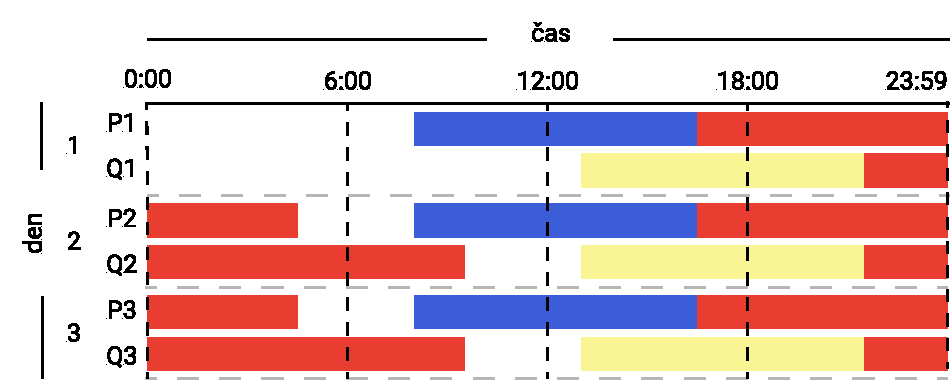
\includegraphics[scale=0.7]{img/shift-overlap.pdf}
	\caption{Nepřekrývání směn}
	\label{fig:shiftprecedencefull}
\end{figure}

Pro zjednodušení jsou směny uspořádané do datové struktury naznačené na obr.~\ref{fig:shiftprecedence}, tak, aby bylo možné vyhledávat platné kombinace o~nějaké délce (dané úvazkem zaměstnance), aby se směny nepřekrývaly.

\begin{figure}[h!]
	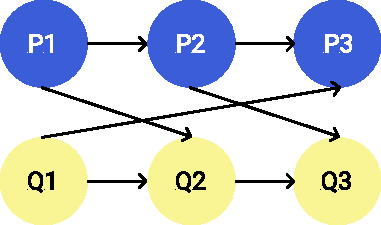
\includegraphics[scale=0.7]{img/shift-overlap-small.pdf}
	\caption{Graf následnosti směn}
	\label{fig:shiftprecedence}
\end{figure}


\section{Délka pracovního týdne}
Předpoklad pro algoritmus je co se týče délky pracovního týdne jednoduchý, neřeší možnost plánování přesčasů. Aby byla dodržena délka pracovního týdne (standardně 40 hodin), případně méně (zkrácené úvazky), každému zaměstnanci se rozvrhne nejvýše \texttt{úvazek $\ast$ 40 / délka směny} směn (zaokrouhleno nahoru). Když se směny ukládají, jedna náhodná z~nich se, je-li to třeba, zkrátí, aby byla délka pracovního týdne dodržena.

\section{Přiřazení na specializovanou směnu}

Pro každou specializovanou směnu existuje směna bez specializace, která probíhá ve stejný čas. Zaměstnanec může být přiřazen na libovolnou nespecializovanou směnu nebo na směnu se specializací odpovídající jeho smlouvě.

\section{Obsazení všech směn}
Tato strategie se pokouší do rozvrhu náhodně vybraných zaměstnanců vložit směnu, která zatím nebyla obsazena, a to způsobem popsaným v~pseudokódu~\ref{lst:noemptyshifts}. Tento algoritmus proběhne pro každou směnu nejvýše $n$-krát.

\begin{lstlisting}[caption={Strategie pro vylepšování obsazení všech směn}, label={lst:noemptyshifts}]
Vyber náhodného zaměstnance
POKUD lze vložit směnu do existujícího rozvrhu
	Vlož směnu do rozvrhu
	Smaž protínající nebo náhodnou směnu z rozvrhu
\end{lstlisting}

\section{Obsazení specializovaných směn}
Tato strategie změní přiřazenou směnu na specializovanou, která probíhá v~daném čase, je-li to možné vzhledem ke specializaci zaměstnance, viz pseudokód~\ref{lst:specialize} (průběh pro jednu směnu v~rozvrhu jednoho zaměstnance).

\begin{lstlisting}[caption={Strategie pro obsazení specializovaných směn}, label={lst:specialize}]
Vyber směnu bez specializace
POKUD probíhá ve stejný čas vhodně specializovaná směna
	Vyměň směnu za specializovanou
\end{lstlisting}

Úspěch této strategie je zaručen u všech směn, pro něž lze nalézt specializovanou směnu, která probíhá ve stejný čas – v~případě, že všechny směny lze specializovat, je sankce za porušení této podmínky vždy nulová. To ale znamená, že některé směny zůstanou zcela prázdné – tedy že naopak tato strategie může zhoršit obsazení všech směn  (je ale otázkou, jestli tento fakt má takovou váhu v~reálném světě a zda vůbec dává možnost \uv{na tuto směnu může přijít kdokoliv} smysl v~případě, že se směny mají rozepisovat s~ohledem na specializaci zaměstnanců).

\section{Více volna v~kuse}\label{sec:freedays}
Postup pro vylepšení, který se aplikuje na rozvrh každého zaměstnance, který zatím nemá 48hodinovou přestávku mezi směnami, je popsán v~pseudokódu~\ref{lst:freedays}. Především tento algoritmus jednu směnu odstraní (tím vytvoří delší volno), a poté se pokusí umístit další směnu mezi dvě jiné.

\begin{lstlisting}[caption={Strategie pro více volna v~kuse}, label={lst:freedays}]
Nalezni 48h přestávku mezi N-1 směnami
Odstraň směnu v tomto časovém období
POKUD lze směnu vložit do druhé největší přestávky
	Vlož směnu do této přestávky
\end{lstlisting}

\section{Obsazení směn úměrně poptávce}
Nalezne se zaměstnanec, který je zapsán na směnu, kde naplnění převyšuje poptávku a $n$ náhodných směn, které poptávku nenaplňují – snahou je vyměnit přeplněnou směnu za prázdnější (pseudokód~\ref{lst:demand}).

\begin{lstlisting}[caption={Strategie pro obsazení směn dle poptávky}, label={lst:demand}]
Vyber náhodného zaměstnance na směnu
POKUD lze tuto směnu vyměnit za méně obsazenou
	Vyměň směnu za méně obsazenou
\end{lstlisting}

\section{Testování}

Při testování heuristických algoritmů nelze kontrolovat, zda byl vrácen jeden konkrétní výsledek (mimo jednoduché případy) a je možné pouze určovat, zda je řešení dost dobré, dost rychlé a validní. Může proběhnout sběr testovacích dat z~místa reálného nasazení algoritmu, případně mohou být data generována náhodně. \cite{rardin2001experimental}

Cílem bylo ověřit na testovacích datech následující předpoklady:
\begin{enumerate}
	\item Algoritmus vrací pro validní vstupy validní řešení.
	\item Strategie snižuje sankci v~daném kritériu.
	\item Čím více strategií, tím je nižší sankce.
	\item Čím více iterací zlepšování, tím lepší řešení.
\end{enumerate}


Pro otestování bylo vytvořeno 8 různých organizací, které se odlišovaly v~počtu zaměstnanců, počtu specializací, pracovní době, počtu směn nebo prioritě směn. Kritérium pro výběr testovacích dat bylo spíše náhodné, pouze byla snaha použít data, která se v~daných parametrech od sebe odlišují. Pro každou organizaci následně proběhlo testování s~různými parametry (počet iterací, váhy kritérií) ve více opakováních.


\subsection{Definice pojmů}
Co se týče prvního předpokladu, řešení bude považováno za validní, pokud algoritmus proběhne bez vyvolání výjimky a bez zacyklení, a pokud se řešení podaří uložit do databáze.

Pro vyhodncení zbývajících předpokladů budou porovnávány průměrné hodnoty ze všech testovacích organizací. Bude-li o~řešení řečeno, že je lepší, znamená to, že je sankce (v~daném kritériu či celkově) nižší než sankce náhodného řešení, na kterém žádné další operace neproběhly (tj. proběhlo 0 iterací vylepšování nebo jsou váhy všech kritérií nulové). Sankce za jedno libovolné porušení dle definice cílové funkce je 1. To znamená, že pokud v~rozvrhu např.~zůstanou tři směny neobsazené, bude sankce 3.

\subsection{Vyhodnocení předpokladů}
Data, o~která se následující vyhodnocování opírá, lze nalézt v~příloze \ref{app:algo-testing}. První předpoklad byl vyvrácen tím, že byla nalezena vstupní data (Organizace G, viz přílohu \ref{app:algo-testing}), pro která může být jak vyvolána výjimka, tak může algoritmus proběhnout korektně (viz~tab.~\ref{tab:errors}). Z~dat vyplývá, že tato chyba nastane, ať už jsou použity strategie na vylepšení rozvrhu či nikoli, to nasvědčuje tomu, že se jedná o~chybu při implementaci vyhledávání směn v~grafu, konkrétně v~případě, že některé směny bez specializace mají nulovou prioritu. V~případě jiných vstupních dat je algoritmus vždy z~tohoto hlediska úspěšný.

\begin{table}[h]
	\caption{Chybovost algoritmu pro organizaci G}
	\label{tab:errors}
	\begin{tabular}{r|rr}
		\hline
		\textbf{Celkem} & \textbf{Korektní} & \textbf{Nekorektní}\\
		\hline
		\rowcolor{Gray}
		617 & 550 & 67\\
		\hline
	\end{tabular}
\end{table}

Co se druhého předpokladu týče, data ukazují, že strategie pro obsazení všech směn není příliš úspěšná v~případě, že se rozvrhují specializované směny~–~data nasvědčují tomu, že rozvrh v~tomto parametru spíše dokáže vylepšit strategie pro obsazení specializovaných směn, když proběhne samostatně, viz~tab.~\ref{tab:empty} udávající průměrné sankce ze všech organizací.

\begin{table}[h]
	\caption{Sankce za obsazení všech směn}
	\label{tab:empty}
	\begin{tabular}{lr}
		\hline
		\textbf{Typ} & \textbf{Průměr}\\
		\hline
		\rowcolor{Gray}
		Náhodné & 15,87\\
		Obs. všech & 15,18 \\
		\rowcolor{Gray}
		Obs. specializovaných & 14,13\\
		\hline
	\end{tabular}
\end{table}

Samotná strategie pro obsazení specializovaných směn je úspěšná~–~sankci oproti náhodnému řešení snižuje ve všech případech výrazně, viz tab.~\ref{tab:specialized}.

\begin{table}[h]
	\caption{Sankce za obsazení specializovaných směn}
	\label{tab:specialized}
	\begin{tabular}{lr}
		\hline
		\textbf{Typ} & \textbf{Průměr}\\
		\hline
		\rowcolor{Gray}
		Náhodné & 43,19\\
		Obs.~specializovaných & 25,06 \\
		\hline
	\end{tabular}
\end{table}

Strategie pro obsazení směn úměrně poptávce je mírně úspěšná, viz tab.~\ref{tab:demand}.

\begin{table}[h]
	\caption{Sankce za obsazení specializovaných směn}
	\label{tab:demand}
	\begin{tabular}{lr}
		\hline
		\textbf{Typ} & \textbf{Průměr}\\
		\hline
		\rowcolor{Gray}
		Náhodné & 54,11\\
		Obs.~úměrně poptávce & 49,96 \\
		\hline
	\end{tabular}
\end{table}

Strategie, která má zajišťovat více dní volna v~kuse, je úspěšná, pokud probíhá izolovaně, nikoli však v~kombinaci s~dalšími strategiemi (viz~tab.~\ref{tab:free}), nebyla však dostatečně testována varianta, kdy je váha tohoto kritéria vyšší oproti ostatním.

\begin{table}[h]
	\caption{Sankce pro více volna v~kuse}
	\label{tab:free}
	\begin{tabular}{lr}
		\hline
		\textbf{Typ} & \textbf{Průměr}\\
		\hline
		\rowcolor{Gray}
		Náhodné & 10,38\\
		Pouze volno v~kuse & 7,36 \\
		\rowcolor{Gray}
		Všechny & 9,38\\
		\hline
	\end{tabular}
\end{table}


Druhý předpoklad tak spíše platí v~případě obsazení specializovaných směn, v~případě strategie pro více volných dní v~kuse a~v~případě obsazování směn úměrně poptávce. Bylo by třeba zrevidovat způsob, jakým je implementována strategie pro obsazení volných směn, aby správně obsazovala i~směny se specializací.%, a zároveň navrhnout odlišný způsob, jak zajišťovat, že mají zaměstnanci více volna v~kuse~–~například by bylo možné zkusit přesouvat směny více.

Třetí předpoklad data spíše prokazují, sankce je u jednotlivých kritérií nižší, pokud dané vylepšování proběhne, výjimkou může být případ po sobě jdoucích dnů volna, zdá se ale, že jiné strategie se mezi sebou neovlivňují negativně, spíše se naopak podporují.

\begin{table}[h]
	\caption{Průměrné sankce po proběhnutí všech strategií}
	\label{tab:iterations}
	\begin{tabular}{lrr}
		\hline
		\textbf{Kritérium} & \textbf{Náhodné} & \textbf{Vylepšované}\\
		\hline
		\rowcolor{Gray}
		Obs. všech & 15,87 & 11,99\\
		Obs. úměrně poptávce & 54,11 & 41,31 \\
		\rowcolor{Gray}
		Obs. specializovaných & 43,19 & 22,38\\
		Volno v~kuse & 10,38 & 9,38\\
		\hline
	\end{tabular}
\end{table}

Co se týče čtvrtého předpokladu, data jednoznačně prokazují, že řešení po jedné iteraci je lepší než náhodné řešení, jiný jasný závěr by si ale vyžádal přesnější posouzení. Získaná data mírně nasvědčují tomu, že toto tvrzení z~hlediska všech sankcí platí (je patrný velmi mírný pokles součtu průměrných sankcí všech řešení pro všechny organizace, viz~tab.~\ref{tab:iterations}), ale rozdíl mezi tím, zda proběhne jedna iterace či více iterací je nevýrazný. Lze předpokládat, že řešení začne velmi brzy konvergovat, tedy že už další zlepšování rozvrhu těmito operacemi nebude dávat smysl.

\begin{table}[h]
	\caption{Součet sankcí při různém počtu opakování}
	\label{tab:iterations}
	\begin{tabular}{lrrrrr}
		\hline
		\textbf{Iterací} & 0 & 1 & 2 & 3 & 4\\
		\hline
		\rowcolor{Gray}
		\textbf{Součet} & 988,54 & 830,86 & 812,83  & 807,90 & 803,22\\
		\hline
	\end{tabular}
\end{table}

\section{Vyhodnocení algoritmu}

Byl navržen triviální algoritmus na rozdělení předem určených směn mezi zaměstnance s~různě velkým úvazkem. V~případě budoucího použití by bylo třeba dále jej vylepšit (především revidovat, které situace byly při implementaci opomenuty) a vzít v~potaz, co by od rozvrhovacího algoritmu očekával ten, kdo by jej využival~–~skoro jistě by se jednalo o~složitější optimalizační úlohu, která by vyžadovala odlišný model.

Z~testování na několika vybraných \uv{organizacích} vyplynulo, že algoritmus není bezchybný, je však schopen ve většině případů generovat rozvrhy, které dávají smysl vzhledem k~nezbytným podmínkám, a navíc je i lehce upravit, aby lépe naplňovaly zbytné podmínky, tedy aby řešení bylo kvalitnější.

\chapter{Implementace}

\section{Architektura aplikace}

Při implementaci byla použita třívrstvá architektura (klient, aplikační server, databáze), jak je naznačeno na obr.~\ref{fig:architecture}. Klientem zde je mobilní aplikace, která komunikuje se serverem přes jeho \acrshort{rest} \acrshort{api}.

\begin{figure}[h]
	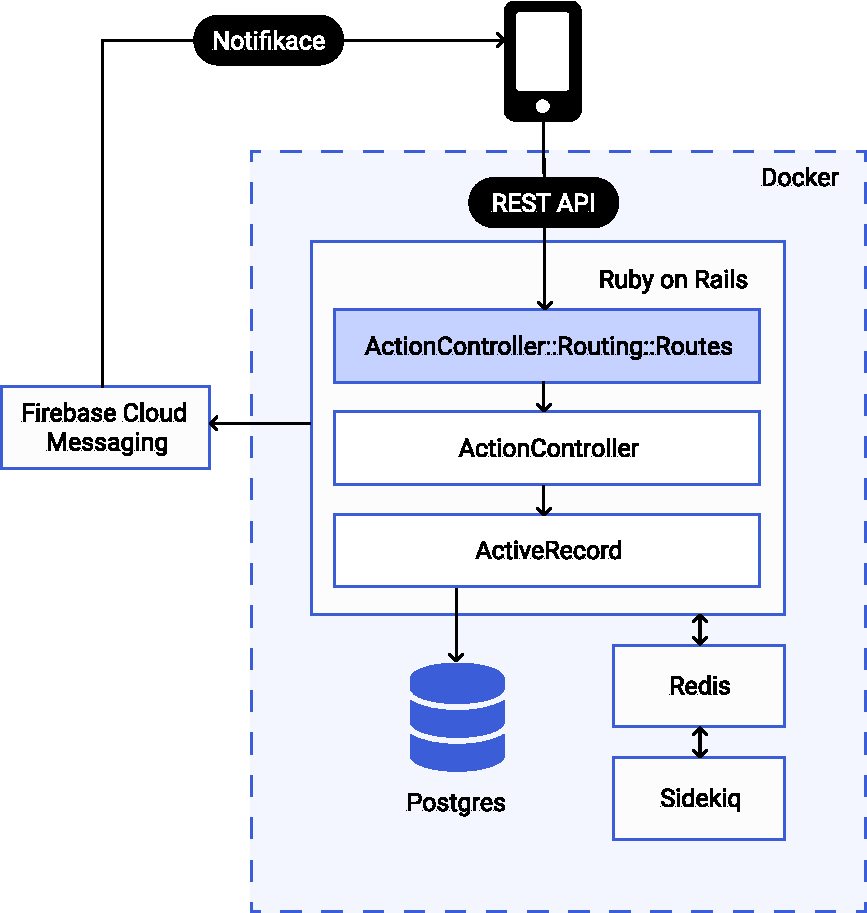
\includegraphics[scale=0.7]{img/architecture.pdf}
	\caption{Architektura aplikace}
	\label{fig:architecture}
\end{figure}


Serverová aplikace běží v~Dockeru z~důvodu snazšího nasazení na různá prostředí, kromě samotné Rails aplikace a databáze jsou v~Dockeru se používají i~služby Redis a~Sidekiq, a to z~důvodu zpracování operací na pozadí, v~této aplikaci jde především o~pravidelné~vytvoření nového týdne pro rozvrhnutí nebo zveřejnění rozvrhu v~případě, že to vedoucí neudělá v~dostatečném předstihu.

Mimo tuto strukturu stojí Firebase Cloud Messaging, který se používá pro posílání notifikací (např.~o~zveřejnění nového rozvrhu nebo nového týdne na naplánování) do mobilní aplikace, když si toto server vyžádá.

Pro více informací o~implementaci viz přílohu \ref{app:analysis}, která obsahuje diagram komponent a~diagram nasazení.


\section{Backend}

Backendová aplikace využívá architektonický vzor \acrshort{mvc}, přičemž uživatelské rozhraní není součástí webové aplikace.

Byla snaha implementovat aplikaci co nejjednodušším způsobem tak, aby v~co největší míře byly dodrženy konvence a nebylo třeba ji příliš konfigurovat~–~controllery jsou implementovány na základě konvencí (viz~kód~\ref{lst:railsconventions}~–~po zavolání cesty \texttt{GET /periods/:id} se automaticky provolá metoda \texttt{show}), není-li nutné to udělat jinak.

\begin{lstlisting}[language=Ruby,caption={Konvenční ActionController}, label={lst:railsconventions}]
class SchedulingPeriodController < ActionController
	def show
			period = SchedulingPeriod.find(params[:id])
			render json: period
	end
end
\end{lstlisting}

Model je implementován s~pomocí objektově relačního mapování, které se stará o~přístup k~databázi. Diagram tříd backendu je součástí přílohy \ref{app:analysis}, Android aplikace přistupuje k~obdobně strukturovaným datům.

Mimo strukturu specifickou pro webovou aplikaci stojí \texttt{Service} třídy, které se provolávají v~případě, že je vhodné některé akce, které nejsou triviální, odsunout mimo controller, a také pomocné datové struktury a strategie pro rozvrhování směn.

Používají se především gemy\footnote{Gem je termín pro knihovny v~Ruby.} Devise Token Auth (autentizace uživatele s~pomocí tokenů), CanCanCan (zabezpečení operací se zdroji na základě uživatelské role) nebo will paginate (stránkování zdrojů).

\section{Mobilní aplikace}

Mobilní aplikace byla navrhnuta dle zásad nejpoužívanějšího a ze strany Googlu doporučovaného architektonického vzoru \acrshort{mvvm}, viz~obr.~\ref{fig:mobile-app}. Při implementaci byly využity především knihovny Koin (pro dependency injection), Retrofit (\acrshort{http} klient) a dále některé součásti Android Jetpack (soubor knihoven pro platformu Android, které usnadňují vývoj udržitelných aplikací a poskytují kompatibilitu se staršími verzemi \acrshort{os} \cite{android2020jetpack}), a to především LiveData (pozorovatelná data respektující životní cyklus Android \acrshort{ui} komponent), Navigation (navigace mezi fragmenty aplikace), DataBinding (propojení \acrshort{ui} komponent definovaných v~\acrshort{xml}~layoutech s~daty), Paging (stránkování seznamů) nebo Room (nadstavba nad databázi SQLite pro perzistenci dat).

\begin{figure}[h]
	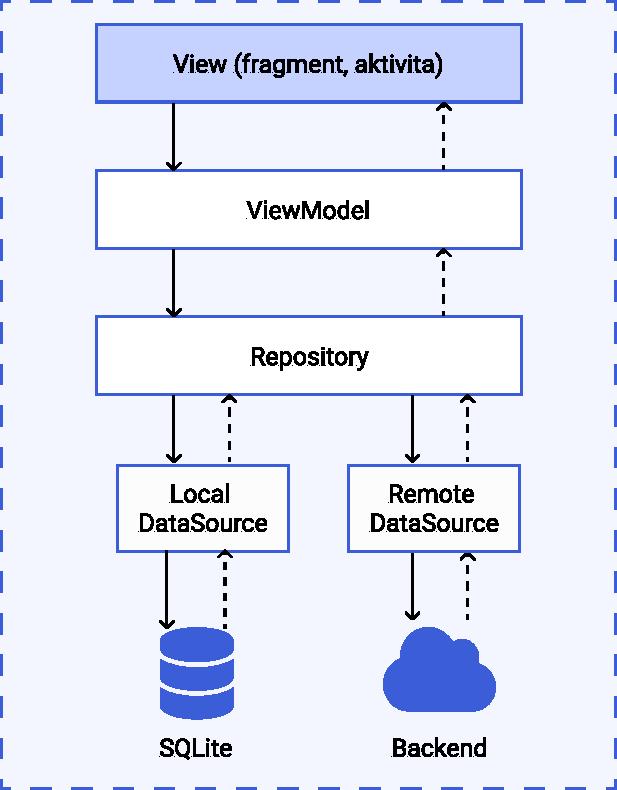
\includegraphics[scale=0.7]{img/mobile-app.pdf}
	\caption{Návrh mobilní aplikace}
	\label{fig:mobile-app}
\end{figure}

Jedná se o~aplikaci s~nižším počtem aktivit (samostatné aktivity se využívají v~případě, že by nebylo vhodné zobrazovat v~aplikaci spodní navigaci, tedy především tehdy, když uživatel vyplňuje formulář, např.~přidává nového zaměstnance), v~níž navigace probíhá s~pomocí Jetpack Navigation (např. detaily směn tedy nejsou sa\-mos\-tat\-ný\-mi aktivitami, ale jedná se o~fragmenty v~aktivitě \texttt{MainActivity}). Většina obrazovek má kromě fragmentu a patřičného layoutu také vlastní ViewModel, existují i~sdílené ViewModely pro přenos dat v~rámci jedné aktivity. Pro ukázku navigačního grafu viz obr.~\ref{fig:navigation-graph}, konkrétně je zde vyobrazena navigace v~aktivitě pro přidávání pracovních dní. Obecně navigace v~aplikaci probíhá v~souladu s~hierarchickým popisem, který je součástí přílohy \ref{app:analysis}.

\begin{figure}[h]
	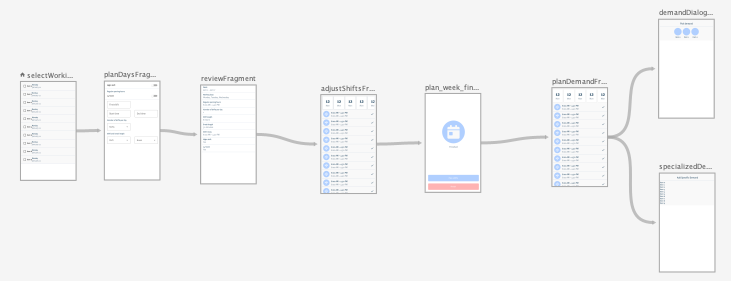
\includegraphics[width=\textwidth]{img/navigation-component.png}
	\caption{Ukázka navigačního grafu}
	\label{fig:navigation-graph}
\end{figure}

\subsection{View}

View je část aplikace, která vykresluje uživatelské rozhraní, může se jednat o~layouty ve formátu \acrshort{xml}, aktivity (základní okno pro \acrshort{ui}) nebo fragmenty (znovupoužitelné). Má referenci na ViewModel a pozoruje jeho změny, podle čehož aktualizuje \acrshort{ui}; při událostech na uživatelském rozhraní (např.~stisknutí tlačítka) může provolat ViewModel.

Pro zjednodušení se používá data binding, pro vytváření nových aktivit byla vytvořena abstraktní třída \texttt{BindingActivity<B: ViewDataBinding>}, pro vytvoření aktivity s~layoutem bez dalších parametrů tak dostačuje kód \ref{lst:newactivity}. Abstraktní aktivita nastaví layout a binding, který je pro potomky přístupný jako proměnná \texttt{binding}, a~nastaví mu vlastníka životního cyklu.

Třída \texttt{ViewModelActivity<V: BaseViewModel, B:  ViewDataBinding>} je abstraktním potomkem \texttt{BindingActivity}, který je přípraven pro aktivity, které mají vazbu na ViewModel (parametry konstruktoru jsou layout a třída ViewModelu). Tato aktivita zajišťuje vytvoření ViewModelu (který se uloží do proměnné \texttt{viewModel} a navíc se nastaví jako parametr pro binding).

\begin{lstlisting}[language=Kotlin,caption={Vytvoření jednoduché aktivity},label={lst:newactivity}]
class SetupActivity :
	BindingActivity<ActivitySetupBinding>(R.layout.activity_setup)
\end{lstlisting}

Velmi podobně jako \texttt{BindingActivity} a \texttt{ViewModelActivity} fungují také abstraktní fragmenty, tj. \texttt{BindingFragment} a \texttt{ViewModelFragment}.

Vzhledem k~použití knihovny LiveData (pozorovatelná data závislá na životním cyklu aktivity/fragmentu) zde větší míře použit návrhový vzor Observer, View pozoruje změny ViewModelu a podle toho se mění obrazovky.

\subsection{ViewModel}

ViewModel je prostředníkem mezi aktivitou a~modelem -- provolává nižší vrstvu a na základě dat, která mu vrátí, mění stav svých proměnných.

ViewModely jsou v~této aplikaci potomkem abstraktní třídy \texttt{BaseViewModel}, která v~sobě obsahuje odkazy na všechny repositáře (inicializace probíhá s~pomocí dependency injection, viz~kód~\ref{lst:viewmodel}); také obsahuje LiveData pro zobrazování chyb a metody pro zpracování chyb, případně dat (to vše proto, aby se méně opakoval stejný kód). ViewModel ukládá odpovědi z~repozitářů jako LiveData.

\begin{lstlisting}[language=Kotlin,caption={Třída \texttt{BaseViewModel}},label={lst:viewmodel}]
abstract class BaseViewModel : ViewModel() {
    protected val userRepository by inject(UserRepository::class.java)
    protected val shiftRepository by inject(ShiftRepository::class.java)
		[...]
}
\end{lstlisting}

\subsection{Model}
Model se skládá z~repozitářů, které mají zodpovědnost za provolávání datových zdrojů (lokálních či vzdálených) a za ukládání dat do databáze či do cache, takto poskytuje požadovaná data. Z~repozitářů se data vracejí obalená ve třídě \texttt{ResponseModel<T>}, ta může nést zprávu o chybě (která se dále zpracují a zobrazí na \acrshort{ui}) nebo požadovaná data.

\begin{lstlisting}[language=Kotlin,caption={Třída \texttt{ResponseModel}},label={lst:responsemodel}]
sealed class ResponseModel<T> {
	class SUCCESS<T>(var data: T? = null, val headers: Headers? = null): ResponseModel<T>()

	class ERROR<T>(val errorType: ErrorType? = null): ResponseModel<T>()
}
\end{lstlisting}

Většinu dat nedává smysl uchovávat v~lokální databázi~–~ukládají se především rozvrhy směn pro zaměstnance, které jsou považovány za natolik důležité, že by měly být dostupné vždy (primárně se stahují aktuální data ze serveru, pokud to není možné, čte se z~databáze).

\subsection{Design}\label{design}

Design aplikace vznikl v~souladu se základními pravidly pro tvorbu uživatelského rozhraní Android aplikací, jak jsou popsány v~Material Design Guidelines\footnote{https://material.io/design/guidelines-overview}, snahou bylo vytvořit minimalistické uživatelské rozhraní, v~němž uživatelé snadno najdou to, co je pro ně důležité. Pro ukázku viz~obr.~\ref{fig:design}, konkrétní návrhy jednotlivých obrazovek jsou v~příloze \ref{app:analysis}.

\begin{figure}[h]
	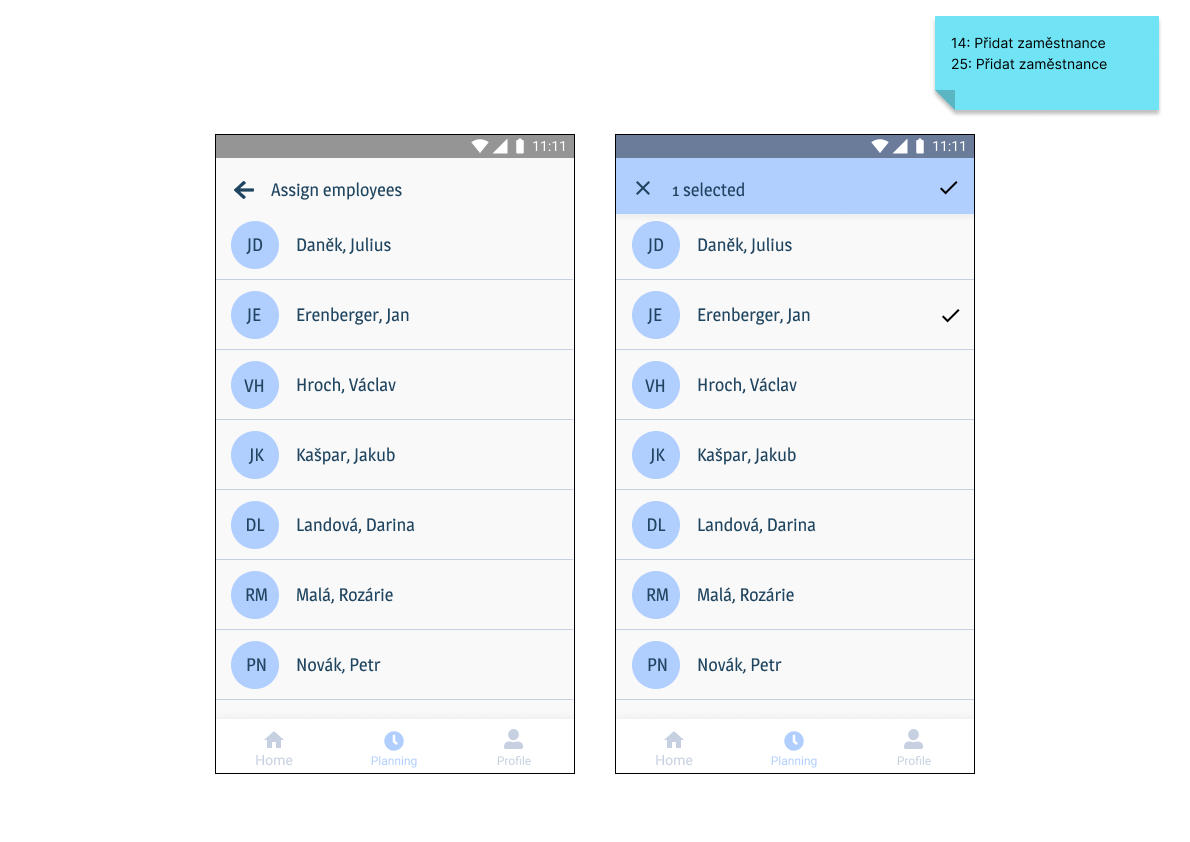
\includegraphics[width=\textwidth]{img/design.png}
	\caption{Výběr zaměstnanců}
	\label{fig:design}
\caption{Ukázka designu}
\end{figure}

Návrh vznikl v~nástroji Figma, ikonky byly převzaty z~knihoven Font Awesome 5 a Material Design Icon.

\subsection{Uživatelské rozhraní aplikace}

Konkrétní snímky obrazovky z~mobilní aplikace jsou na obr.~\ref{fig:screenshots} (pro více snímků obrazovky viz předpokládáný průchod aplikací v~příloze \ref{app:user-testing}).

\begin{figure}
	\begin{subfigure}{0.34\textwidth}
				 %\centering
				 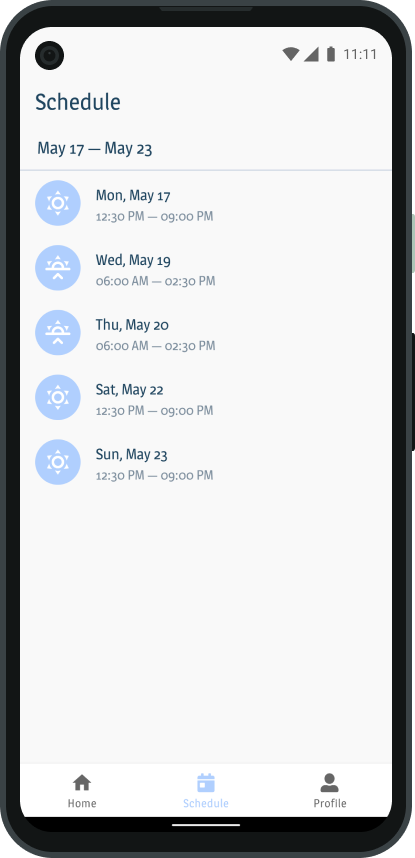
\includegraphics[width=\textwidth]{img/schedule.png}
				 \caption{Rozvrh směn}
				 \label{sub:android1}
  \end{subfigure}
		 \hspace{1em}
	\begin{subfigure}{0.34\textwidth}
				 %\centering
				 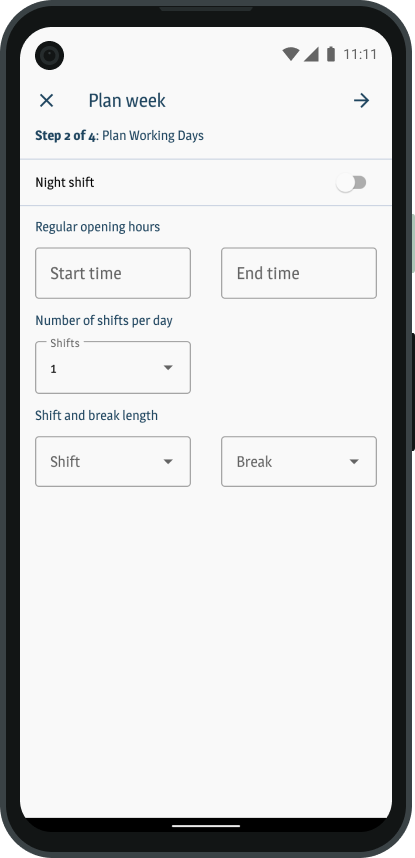
\includegraphics[width=\textwidth]{img/plan-week.png}
				 \caption{Plánování týdne}
				 \label{sub:android2}
  \end{subfigure}
	\vspace{1em}
	\begin{subfigure}{0.34\textwidth}
         %\centering
         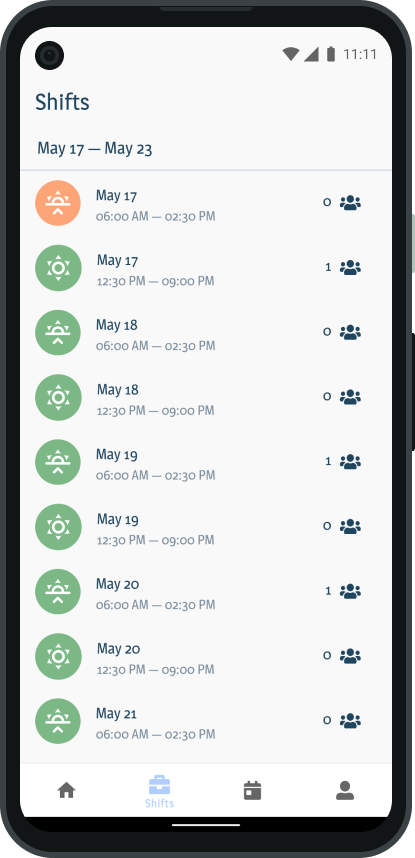
\includegraphics[width=\textwidth]{img/empty-shifts.png}
         \caption{Volné směny}
         \label{sub:android3}
     \end{subfigure}
		 \hspace{1em}
	\begin{subfigure}{0.34\textwidth}

         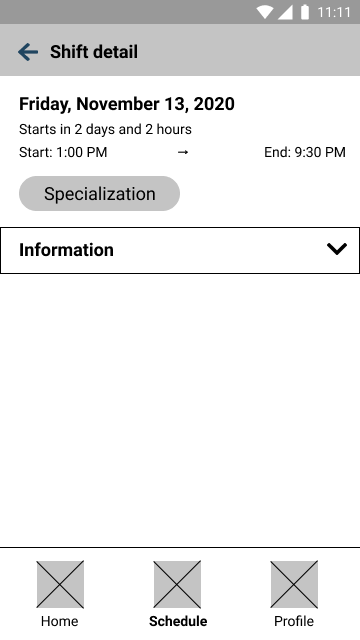
\includegraphics[width=\textwidth]{img/shift-detail.png}
         \caption{Detail směny}
         \label{sub:android4}
     \end{subfigure}
	\caption{Snímky obrazovky z~Android aplikace}
	\label{fig:screenshots}
\end{figure}

\chapter{Uživatelské testování}

\section{Způsob testování}
Testování proběhlo jako odlehčená verze testu použitelnosti, probíhalo vzdálenou formou. Účastníkům byl předem poskytnut popis jednotlivých pojmů (viz~přílohu \ref{app:analysis}) a instrukce popisující, co se od nich chce a~na co se mají konkrétně zaměřit, dále testovací scénáře, kterými měli projít (viz přílohu \ref{app:user-testing}). Testování bylo kvalitativní, proběhlo na třech účastnících, což je dle \cite{nielsen2000why} optimální počet, aby byly od~uživatelů získávány nové podněty. Účastníci byli vybráni dle příslušnosti k~cílové skupině či dle znalosti problematiky.

Před testováním byl sestaven předpoklad o~průchodu aplikací ve formě po sobě následujících snímků obrazovky, který je součástí přílohy \ref{app:user-testing}. Zpráva z~testování, obsahující podrobnosti o~průchodu uživatelů aplikací, je součástí přílohy \ref{app:user-testing}.

\section{Průchod aplikací}
Všichni uživatelé aplikaci prošli podle doporučeného scénáře, před tím si přečetli instrukce a popis aplikace a potvrdili, že všemu rozumí a dává jim to smysl. Při průchodu většinou testovacích scénářů neměli zásadní problémy, aplikace jim připadala intuitivní.

Největším zádrhelem se ukázalo být přihlašování, především uživatelům chyběla možnost obnovit si heslo či si jej zkontrolovat při vyplňování, také jim scházela možnost upravit špatně odeslaná data (smluvy, specializace, uživatelské údaje). Jako matoucí působil průvodce rozvrhováním pracovní doby na daný týden~–~toto muselo být více vysvětleno, aby se dokázali zorientovat.

\section{Návrhy na zlepšení}
Z~rozhovorů s~potenciálními uživateli vyplynula celá řada návrhů na zlepšení aplikace. Byly rozděleny do dvou kategorií~–~připomínky k~implementaci aktuálních funkcionalit a~návrhy do budoucna (toto rozdělení návrhů je pouze orientační).

\subsection{Aktuální aplikace}
\begin{itemize}
	\item Překlad aplikace do češtiny,
	\item změna rozložení či barev tlačítek v~registračním formuláři,
	\item zvýraznění prvků uživatelského rozhraní,
	\item změna textu některých tlačítek,
	\item lepší zpětná vazba při zveřejnění rozvrhu,
	\item plánování rozvrhu na měsíc, nikoli na týden,
	\item úprava chybových hlášek, aby byly konkrétnější,
	\item označení povinných a nepovinných polí formuláře.
\end{itemize}

\subsection{Návrhy do budoucna}
\begin{itemize}
	\item Umožnění úpravy rozvrhu po zveřejnění (\textit{\uv{Co když někdo třeba onemocní?}}),
	\item umožnění úpravy odeslaných dat,
	\item zobrazení kontaktů na uživatele zaměstnancům, přidání telefonního čísla,
	\item zobrazení rozvrhu ve formě tabulky, nejen seznamu,
	\item zobrazení celkového rozvrhu všem zaměstnancům,
	\item podpora platformy iOS.
\end{itemize}


\section{Vyhodnocení}
Uživatelé aplikací prošli v~předpokládaném sledu obrazovek. Shodli se na tom, že by ji dokázali používat, myslí si, že by se s~ní naučili a zvykli by si. Ocenili její jednoduchost, snadnost ovládání i to, že se zobrazují pouze informace, které jsou relevantní. Celkové hodnocení je pozitivní, navíc byla poskytnuta řadu návrhů na zlepšení, které by bylo vhodné vzít v~potaz, pokud by vývoj dále pokračoval.


\chapter*{Závěr}

V~této práci byl představen způsob, jakým by bylo možné vylepšit interní procesy organizace, která rozvrhuje směny svým zaměstnancům na základě sady různých pravidel, ať už vyplývají z~legislativy, personální situace ve firmě nebo z~manažerských požadavků, a to prostřednictvím jednoduché mobilní aplikace, která bude dostupná jak vedoucím, tak zaměstnancům.

V~úvodní kapitole teoretické části bylo popsáno plánování pracovních sil z~hlediska manažerského rozhodování (jaké faktory jej mohou ovlivnit) a z~hlediska legislativního, kdy je třeba rozvrhovat s~ohledem na stanovenou týdenní pracovní dobu, s~ohledem na druh pracovněprávního vztahu nebo s~ohledem na přestávky mezi směnami.

Ve druhé kapitole dále byly popsány některé teoretické metody, které jsou vhodné pro optimalizaci rozvrhů směn na základě rozhodujích faktorů~–~může se jednat o~tradiční deterministické metody pro optimalizaci cílové funkce, případně o~metaheuristiky, které se přizpůsobí problému rozvrhování směn.

Ve třetí kapitole byla vytvořena představa o~organizacích cílové skupiny, na základě toho byly sestaveny požadavky na novou aplikaci, která by zjednodušila interní procesy týkající se rozvrhování směn.

Ve čtvrté kapitole bylo popsáno rozhodování o~technologiích pro implementaci uživatelského rozhraní a~serverové části aplikace, na základě toho byly stanoveny požadavky na kvalitu software.
% ve formě mobilní aplikace, která umožňuje lépe plánovat směny (ať už automaticky nebo manuálně).

V~páté kapitole byl přiblížen návrh algoritmu, který se v~této aplikaci používá pro automatické rozvrhování směn~–~tento algoritmus byl inspirován již existujícími teoretickými metodami, a tak se rozvrhuje na základě řady podmínek, které byly rozděleny na zbytné a~nezbytné. Nezbytné mají za úkol kontrolovat, zda řešení dává smysl z~hlediska legislativy (zda má dostatečnou přestávku), případně obecně (zda například zaměstnanec nemá být na dvou místech zároveň), zbytné určují kvalitu na základě požadavků manažerů (vždy je někdo na pracovišti) a~zaměstnanců (volné dva dny v~kuse).

Šestá kapitola popisovala způsob, jakým je navržená aplikace implementována, a to jak její backendová část, pro kterou byl použit webový framwork Ruby on Rails, aby byl vývoj v~co největší míře usnadněn, tak i~Android aplikace, která se snaží v~co největší míře použít moderní postupy vývoje.

Poslední kapitola byla věnována uživatelskému testování, které jak potvrdilo vůli potenciálních uživatelů takovou aplikaci používat, tak přineslo řadu nových návrhů, které uživatele při průchodu aplikací napadaly.

Cíl práce, jímž byla analýza, návrh a implementace mobilní aplikace pro plánování lidských zdrojů, byl celkově naplněn, aplikace byla otestována na několika potenciálních uživatelích, kteří vyjádřili ochotu podobnou aplikaci využívat, poskytli pozitivní zpětnou vazbu a~řadu návrhů, které by bylo vhodné zapracovat v~případě, že by práce byla dále rozšiřována.

Prokázalo se tak, že by bylo možné takovou podpůrnou aplikaci pro rozvrhování vyvinout, obzvlášť pokud by se jednalo o~komerční projekt, který byl měl větší rozpočet, více času a větší tým analytiků a vývojářů. V~tom případě by bylo vhodné aplikaci rozšířit a dále vylepšit na základě důkladnějšího sběru požadavků od~všech zúčastněných stran.

Druhou důležitou součástí této práce byl návrh vlastního algoritmu pro rozvrhování směn mezi zaměstnance, způsob jeho implementace reflektuje fakt, že se jedná pouze o~součást bakalářské práce, je tedy navržen v~triviální podobě, která není zdaleka připravená na reálné nasazení, přesto byl i~tento cíl, tedy umožnit v~aplikaci automatické rozvrhování směn na základě vybraných podmínek, naplněn. Pokud by měl být systém, který umožňuje automatické rozvrhování, nasazen v~reálném prostředí, bylo by třeba zohlednit daleko větší množství podmínek~a~požadavků, a algoritmus jim přizpůsobit.

Na tomto místě je vhodné podotknout, že systém pro rozvrhování pracovních sil zcela určitě nestojí ve vakuu, ale naopak řeší problém, který je ryze praktický, a setkává se s~ním řada potenciálních uživatelů ve~svém každodenním životě. Softwarové řešení dává smysl, ale realita je vždy složitější, než aby šlo všechny varianty, které mohou nastat, ať už z~hlediska legislativy, tak z~hlediska lidského faktoru, pokrýt aplikací, kterou vývojáři musí připravit v~konečném čase.

Součástí této práce je řada příloh, které obsahují kromě samotných zdrojových kódů aplikací (mobilní a webové) také podrobnější analýzu, návrh uživatelského rozhraní nebo výsledky testování.



\printbibliography[title={Seznam použité literatury}]

\appendix
\chapter{Dokumenty}

\section{Analýza systému}\label{app:analysis}
\begin{itemize}
	\item Popis pojmů
	\item Diagram tříd
	\item Diagram nasazení
	\item Diagram komponent
	\item Hierarchie obrazovek, wireframes
	\item Návrh uživatelského rozhraní
\end{itemize}

\section{Uživatelské testování}\label{app:user-testing}

\begin{itemize}
	\item Instrukce k~uživatelskému testování
	\item Testovací scénáře
	\item Zpráva z~testování
	\item Předpokládaný průchod aplikací
\end{itemize}

\section{Testování algoritmu}\label{app:algo-testing}

\begin{itemize}
	\item Tabulka s~daty z~testování
\end{itemize}

\chapter{Zdrojové kódy}

\begin{itemize}
	\item Android aplikace
	\item Ruby on Rails aplikace
\end{itemize}

\end{document}
